\documentclass[
  11pt,
  a4paper
]{article}

% ------------------------------ font
% \usepackage{times} pdflatex
\usepackage{luatexja}
\usepackage{luatexja-fontspec}

\setmainfont{Times New Roman}
\setmainjfont[BoldFont=IPAexGothic]{IPAexMincho}

% ------------------------------ math
\usepackage{amsmath,amssymb}
\usepackage{siunitx}

% ------------------------------ author & natbib
\usepackage{authblk}
\usepackage[semicolon]{natbib}
\bibliographystyle{agsm}

% ------------------------------ appendix
\usepackage[title]{appendix}

% ------------------------------ tables
\usepackage{here}
\usepackage{longtable, booktabs, array}
\usepackage{threeparttable, threeparttablex, multirow}
% \newcolumntype{d}{S[input-symbols = ()]}

% ------------------------------- figures
\usepackage{graphics, graphicx}
\makeatletter
\def\maxwidth{\ifdim\Gin@nat@width>\linewidth\linewidth\else\Gin@nat@width\fi}
\def\maxheight{\ifdim\Gin@nat@height>\textheight\textheight\else\Gin@nat@height\fi}
\makeatother
% Scale images if necessary, so that they will not overflow the page
% margins by default, and it is still possible to overwrite the defaults
% using explicit options in \includegraphics[width, height, ...]{}
\setkeys{Gin}{width=\maxwidth,height=\maxheight,keepaspectratio}

% ------------------------------ page settings
\usepackage[left=3cm,right=3cm,top=3cm,bottom=3cm]{geometry}
\usepackage{setspace}
\renewcommand{\baselinestretch}{1.5}
\providecommand{\tightlist}{%
  \setlength{\itemsep}{0pt}\setlength{\parskip}{0pt}}

% ------------------------------ hyperlink
\usepackage{hyperref}

% ------------------------------ other packages
\renewcommand\Affilfont{\itshape\small}
\usepackage{booktabs}
\usepackage{siunitx}

  \newcolumntype{d}{S[
    input-open-uncertainty=,
    input-close-uncertainty=,
    parse-numbers = false,
    table-align-text-pre=false,
    table-align-text-post=false
  ]}
  

% ------------------------------ paper information
\title{Only You:
A Field Experiment of Text Message to Prevent Free-riding in Japan Marrow Donor Program\thanks{In conducting this study, we would like to thank the Japan Marrow Donor Program Office for managing of the field experiment and providing us with the data. This study was conducted with the approval of the institutional review board of the Graduate School of Economics, Osaka University (approval number: R030305-2) and the Japan Marrow Donor Program (approval number: JMDP2021-04). Funding: This work was supported by the Japan Society for the Promotion of Science {[}grant number 20H05632 (F., Ohtake, H., Kato){]} and the Ministry of Health, Labour and Welfare {[}grant number 19FF1001 (F. Ohtake, S., Kurosawa, T., Fukuda){]}.}}
\author[a]{%
  Hiroki Kato\thanks{Present Address: 2-1 Naka, Kunitachi, Tokyo 186-8601, Japan (Hitotsubashi Institute for Advanced Study, Hitotsubashi University). E-mail address: \href{mailto:hkato.econ@r.hit-u.ac.jp}{\nolinkurl{hkato.econ@r.hit-u.ac.jp}}}
}
\author[b]{%
  Fumio Ohtake
}
\author[c]{%
  Saiko Kurosawa
}
\author[d]{%
  Kazuhiro Yoshiuchi
}
\author[e]{%
  Takahiro Fukuda
}
\affil[a]{Graduate School of Economics, Osaka University}
\affil[b]{Center for Infectious Disease Education and Research (CiDER), Osaka University}
\affil[c]{Department of Oncology, Ina Central Hospital}
\affil[d]{Graduate School of Medicine, Tokyo University}
\affil[e]{Department of Hematopoietic Stem Cell Transplantation, National Cancer Center Hospital}
\date{Last updated on December 15, 2023}

\begin{document}
\maketitle
\begin{abstract}
Only half of the patients registered with the Japan Marrow Donor Program receive allogeneic hematopoietic stem cell transplantation because much of the transplant coordination is interrupted due to the reluctance of registered donors to donate. In collaboration with the Japan Marrow Donor Program, we conducted a field experiment to test an information provision intervention for increasing registered donors' willingness to donate. We found that information about the low number of potential donor matches per patient increased the willingness to donate by 25\% among men in their 20s. We also found that knowing that early coordination increases a patient's transplant rate encourages women in their 20s to respond early. These results suggest that providing information affects only certain genders and ages and encourages behavioral change among younger donors with better transplant outcomes.
\vskip\baselineskip
\noindent
\textit{JEL classification}: D64, D90, H41, I11
\vskip\baselineskip
\noindent
\textit{Keywords}: Japan Marrow Donor Program, field experiment, text message, information provision, free-riding, present bias
\end{abstract}



\hypertarget{intro}{%
\section{Introduction}\label{intro}}

Allogeneic hematopoietic stem cell transplantation (HSCT) is one of the treatments with the lowest relapse rates for leukemia and other blood diseases. In this treatment, (1) anticancer drugs and radiation simultaneously kill tumor cells and healthy hematopoietic stem cells, and (2) healthy hematopoietic stem cells donated by others are transplanted. Transplantation requires that the donor's white blood cell type, called HLA, match the patient's HLA.\footnote{In recent years, transplantation between close relatives with semi-matched HLA, known as haploidentical stem cell transplantation, has become more common. In addition, transplantation of blood cells from the umbilical cord or placenta that connects mother and child (cord blood transplantation) has also increased. Unlike bone marrow transplantation, cord blood transplantation can be performed even if the HLA is not a perfect match. In Japan, bone marrow (or peripheral blood) transplants between unrelated individuals ( the focus of this study), will account for 20\% of all transplants performed in FY2021 \citep{JapaneseDataCenterf2022}.} Whereas the probability of a match between two randomly selected individuals is less than 1\%, the probability of a match between siblings is the highest at approximately 30\%. The probability of a match between parents and their children is also low.

If there is no match among relatives, patients must seek a nonrelative donor. In Japan, patients usually seek nonrelative donors through the Japan Marrow Donor Program (JMDP). However, coordination through the JMDP takes a long time, and only 60\% of registered patients receive transplants \citep{Hirakawa2018}. Therefore, it is important to shorten the time to transplantation and increase the transplantation rate in registered patients.

There are two types of donor pool policies that increase transplantation rates. The first includes policies that increase the number of potential donors to increase the probability of a match. Compared with patients matched with fewer than four donors, the transplantation rate increased from 45\% to 74\% for patients matched with more than 200 donors \citep{Hirakawa2018}. However, according to \citet{Takanashi2016}, the probability of a first-time match increased by only 5\%, even though the number of potential donors nearly doubled between 2000 and 2015.\footnote{This is because the probability of a new donor with a rare HLA type is low.} The marginal benefit of increasing the number of potential donors is small.

The second intervention increases the proportion of potential donors willing to donate and improves the quality of the donor pool. \citet{Hirakawa2018} found that many coordinations (73\% of those conducted in 2004--2013) were interrupted before the first process of coordination, confirmatory typing, for donor-related reasons (including poor health). Younger donors are less likely to interrupt coordination for health reasons and more likely to interrupt coordination for other personal reasons, such as lack of motivation.\footnote{While 15\% of males men in their 20s were suspended due to donor health (history, back pain, undergoing treatment, etc.), 41\% were suspended for reasons other than donor health (inability to contact, unavailability, etc.). In addition, 6\% were interrupted due to lack of family consent, a prerequisite for transplantation. The remaining coordinations were either suspended due to patients or reached transplantation.} This is an issue not only in the JMDP but also in marrow donor programs in other countries \citep{Haylock2022}. Given the better transplant outcomes for younger men than for other genders and ages \citep[for example,][]{Kollman2016}, interventions to increase the willingness to donate (especially among younger men) are more important than increasing the donor pool size.

Therefore, this study examines the effect of providing information that increases willingness to donate as one of the measures to improve the quality of the donor pool. When a potential donor registered with the JMDP is matched to a specific patient, the matched donor receives a compatibility notice from the JMDP. Matched donors who respond to the notice by indicating their willingness to donate are coordinated for transplantation. We added two new messages to the compatibility notice based on information published by the JMDP and conducted a field experiment in collaboration with the JMDP to test the effects of the additional messages.

The first message indicates that the number of HLA-compatible donors per patient is low. If there are other potential donors with the same HLA type in the pool, one's donation can be substituted for that compatible donor. In addition, multiple donors (up to 10) can be coordinated with a single patient simultaneously. Thus, transplantation through JMDP is public goods. Donors who gain utility from the patient's survival will be more reluctant to donate the more common the HLA. In other words, JMDP-mediated transplantation faces a standard ``free-ride'' problem \citep{Bergstrom2009}.

This problem is essentially the same as the volunteer dilemma, in which public goods are produced by the cooperative behavior of only one person. In the volunteer dilemma, the theory predicts that the probability of cooperative behavior by even one person decreases with the group size, and this hypothesis has been confirmed by laboratory experiments \citep{Diekmann1985, Diekmann1986, Franzen1999, Davis2017}. Additionally, an interview study of previously matched donors \citep{Kurosawa2022} found that those with low donation intentions felt that they were ``one of several donors,'' implying that the fact that their donation could be substituted by others discouraged them from donating. An important difference from the volunteer dilemma is that potential donors in the JMDP cannot know their own HLA type or the number of matched donors simultaneously; therefore, they cannot accurately estimate the size of the group. Consequently, potential donors may overestimate the number of possible substitutes and may be reluctant to donate. The first message aims to correct the behavior resulting from this misperception.

The second message presents information that early coordination would increase a patient's transplant rate. This message is intended to prevent time-inconsistent donors from delaying their response to the compatibility notice. Time inconsistency is caused by present bias, a key finding of behavioral economics \citep{Laibson1997, ODonoghue2001}.\footnote{Present bias is a phenomenon in which the time discount rate decreases over time. This can cause people to choose low current benefits even if they believe in advance that high future benefits are desirable.} Time-inconsistent donors delay responding, even though they believe in advance that they should respond immediately. The second message shows that the utility of transplantation decreases over time (regardless of the individual's time preference) and aims to change the behavior of the time-inconsistent donor.

Four experimental arms were created to test the effects of the above messages. The first experimental arm sent a compatibility notice without the above two messages to the matched donors (control group). The second and third experimental arms added one of the above messages to the compatibility notice. In the fourth experimental arm, both messages were added to the compatibility notice.\footnote{This experimental arm is designed to test the hypothesis that the simultaneous addition of two intervention messages may cause the matched donor to receive excessive information and suffer from cognitive overload.} We conducted a field experiment with 11,154 matched donors who received compatibility notices between September 2021 and February 2022. Participants were assigned to the experimental arms using weekly cluster randomization. We received coordination data at the end of June 2022, in collaboration with JMDP, to test the effects of the messages.

The experiment found that the intervention messages affected only younger donors with better transplant outcomes.This study has two main findings. First, providing only the information that there are fewer HLA-matched donors per patient increases the willingness to donate and the probability of reaching confirmatory typing among men in their 20s. However, this message has no statistically significant effect on other sexegenders or age groups. Second, providing information that early coordination would increase a patient's transplant rate does not affect the overall response rate for women in their 20s but does increase responses within four days of sending a compatibility notice.\footnote{JMDP recommends a response to the compatibility notice within seven days.} In other words, this information shortens the number of days to respond rather than encouraging response behavior itself. This effect was not observed in the other sexes or age groups.

This study suggests that information can increase the willingness of potential donors to donate and provides practical insights into marrow donor programs worldwide, including the JMDP. Similar to the JMDP, the German-based international marrow donor program, DKMS, and the U.S. marrow donor program, NMDP, have steadily increased their enrollment, but have faced challenges in keeping enrollees motivated and achieving coordination \citep{Switzer1999, Switzer2004, Haylock2022}. Studies have examined the effectiveness of donor leave laws \citep{Lacetera2014} and DKMS's efforts to maintain donor motivation \citep{Haylock2022}.

\citet{Switzer2018} applied an intervention to a message sent by the NMDP when they asked matched potential donors to donate. Their intervention was a message that said, ``Based on the information we currently have, you are in the unique position of likely being a perfect match for this patient.'' This message was delivered over the phone to the potential donor whose HLA was a perfect match. Their experiment was not a fully randomized controlled trial and showed that this novel message did not increase the number of coordination. Although our intervention is very similar to that in this study, we show that the message effect is quite heterogeneous, affecting only certain genders and ages.

In addition, this study contributes to the economic study of costly prosocial behavior such as blood donation. Although stem cell transplantation and blood donation have some similarities, some differences also exist. In the case of blood donation, the time of intention to donate and the time of actual donation are the same, while in the case of stem cell transplantation, the two time points are different. Therefore, maintaining the willingness of potential donors is a challenge for marrow donor programs. Similar to stem cell transplantation, blood donation can be considered public goods. \citet{Wildman2009} used data on blood donors only and showed that free-riding does not occur. In contrast, our study shows that information about the low number of HLA-compatible donors per patient increases the willingness of men in their 20s to donate, suggesting that they overestimate the number of HLA-compatible donors and engage in free-riding.

The remainder of this study is organized as follows: Section \ref{experiment} provides an overview of the coordination process in the JMDP and details the field experiments. Section \ref{result} presents the results, and Section \ref{conclusion} provides a discussion and conclusions.

\hypertarget{experiment}{%
\section{Field Experiment}\label{experiment}}

\hypertarget{background}{%
\subsection{Background: Coordination Process of JMDP}\label{background}}

To better understand the timing of our interventions and our data, we outline the coordination process leading up to the donation of stem cells by potential donors enrolled in the JMDP. First, when a potential donor is matched with a patient enrolled in the JMDP, the JMDP office sends the donor the compatibility notice requesting a stem cell donation.\footnote{At the same time, the JMDP office sends a social networking message to the matched donors informing them that JMDP has sent the compatibility notice.} The matched donor completes a questionnaire and responds to the compatibility notice, indicating their willingness to donate.

Coordination of the transplant begins. The matched donor undergoes confirmatory typing within approximately one month. The coordinator explains the details of the donation process and asks matched donors and their families about their willingness to donate. Matched donors can choose between two collection methods (bone marrow or peripheral blood stem cell collection). In addition, the coordinating physician conducts an interview, medical examination, and blood draws to test for infection and blood type. These tests are performed to determine whether matched donors meet the criteria established by the JMDP.

Patients can be matched with up to 10 compatible donors at one time. The patient's physician selects the most appropriate candidate from matched donors who have undergone confirmatory typing. Importantly, the matched donor does not have access to any information about the matched patient (e.g., the number of other available matched donors). Nor can the matched donor obtain this information from the coordinator or the coordinating physician.

The matched donor, who is selected as the best donor, must give final consent after being informed by the coordinator and coordinating physician. Simultaneously, a representative of the donor's family must consent to the donation. Subsequently, the selected donor cannot change their mind. After the final consent is given, the selected donor admits themselves to hospital for approximately one week to undergo preoperative examinations and preparation for the donation. The donor then undergoes a surgical procedure to collect stem cells. The time from the confirmatory typing to collection is approximately 3 to 4 months.

\hypertarget{design}{%
\subsection{Experimental Design}\label{design}}

Our experiment intervenes in the content of the compatibility notice in which JMDP requests stem cell donation from a matched donor. The standard compatibility notice is as follows:

\begin{quote}
We inform you that your HLA type (white blood cell type) matches that of a patient on our registry and you have been selected as one of our potential donors. We are contacting you to ask if you would like to undergo further testing and interviews in preparation for donation. Please read the enclosed materials carefully, consider whether coordination is possible, and return the form \emph{within 7 days} of receiving this information. {[}Insert intervention messages here{]} If we proceed with the coordination after receiving your return, a coordinator will contact you by phone to discuss the details of your request.
\end{quote}

The donor should respond to the compatibility notice within 7 days. JMDP also encloses a handbook that describes the coordination process outlined in the previous subsection as well as the medical questionnaire and donor consent form.

We added two messages (a probability message and an early coordination message) to the compatibility notice to facilitate coordination.\footnote{In designing our intervention messages, we have been careful to avoid putting undue psychological pressure on potential donors. Specifically, first, we avoid language that sounds like an appeal. Second, we only use information that is publicly available from the JMDP. In addition, the risks of transplantation are explained in the usual way. The intervention message was approved by the Institutional Review Board of the Graduate School of Economics of Osaka University and the JMDP.} The Probability message is as follows:

\begin{quote}
The number of registered donors whose HLA type matches that of a single registered patient is one in hundreds to tens of thousands. We hope you understand that while we may find more than one potential donor, it is not a large number.
\end{quote}

This message emphasizes the low number of matched donors per registered patient. Transplantation is public goods in the sense that, if there are other potential donors with the same HLA type in the pool, one's donation can be substituted for that compatible donor. Thus, as predicted by the volunteer dilemma, the more common the HLA type, the more reluctant the donor will be to donate.

However, in the context of stem cell transplantation, the expectation of the group size influences the decision because a matched donor cannot know the exact size of the group. Therefore, the higher the donor's expectation regarding the number of potential donors with the same HLA type, the more reluctant they will be to donate. If a donor's beliefs are too high, the probability message discourages free-riding and increases willingness to donate by adjusting beliefs downward. The opposite effect may occur. If the donor's beliefs are underestimated, the probability message may induce free-riding and reduce donation intentions by adjusting beliefs upward.

The Early Coordination message is as follows:

\begin{quote}
About 60\% of patients can receive a transplant through the Japan Marrow Donor Program. The earlier a donor can be found to donate bone marrow, the higher that percentage can be.
\end{quote}

This message is expected to work for time-inconsistent matched donors. Time-inconsistent donors may think it is optimal to respond immediately in advance but delay their response. This message suggests that early coordination increases the rate of transplantation for the patient and that the utility of transplantation decays over time (regardless of the individual's time preference). Time-inconsistent donors who read this message may recognize that delaying a response does not increase utility and may change their decision to respond immediately. Thus, this message is expected to increase the response rate over a short period.

Four experimental arms were established to estimate the effects of two intervention messages. Experimental arm A received a standard compatibility notice with no intervention messages (control group). Experimental arms B and C received notices with probability messages and early coordination messages, respectively. Experimental arm D received a notice with two intervention messages added simultaneously. This experimental arm was designed to test the negative effects of the cognitive load caused by information overload.

\begin{table}

\caption{\label{tab:assignment}Assignment Schedule}
\centering
\fontsize{9}{11}\selectfont
\fontsize{9}{11}\selectfont
\begin{threeparttable}
\begin{tabular}[t]{lcccccc}
\toprule
week & Sep 21 & Oct 21 & Nov 21 & Dec 21 & Jan 22 & Feb 22\\
\midrule
Week 1 & B & C & C & D & B & A\\
Week 2 & D & B & A & A & C & B\\
Week 3 & A & D & B & C & D & C\\
Week 4 & C & A & D & B & A & D\\
\bottomrule
\end{tabular}
\begin{tablenotes}
\item Notes: See Table \ref{tab:summary} for detail intervention of each experimental arm. Control group is experimental arm A.
\end{tablenotes}
\end{threeparttable}
\end{table}

The participants in the experiment were 11,154 matched donors who received a compatibility notice between September 2021 and February 2022. To maintain randomness to the best of the JMDP office's abilities, we assigned experimental arms using weekly cluster randomization. The experimental arms were designed to be balanced across weeks and months as much as possible. Table \ref{tab:assignment} summarizes the assignment schedule. Before conducting the experiment, we obtained approval from the institutional review board of the Graduate School of Economics, Osaka University (approval number: R030305) and JMDP (approval number: JMDP2021-04).

\hypertarget{data-and-empirical-strategy}{%
\subsection{Data and Empirical Strategy}\label{data-and-empirical-strategy}}

JMDP provided coordination data at the end of June 2022. The unit of observation is the experimental participant. For individual characteristics, the data recorded gender, age, number of coordination experiences, and prefecture-level residence area. About During the coordination process, the data recorded whether each stage (response to compatibility notice, confirmatory typing, candidate selection, final consent, and collection) was reached. We used these variables as outcome variables. In addition, for responses to the notice, the data recorded the number of days required to respond and the willingness to donate. If coordination was interrupted, the reasons for the interruption were recorded in three categories (patient reasons, donor non-health reasons, and donor health reasons). The analysis uses 11,049 matched donors living in Japan whose coordination (including interruptions) was completed.\footnote{One matched donor lived abroad. There were 104 matched donors with ongoing coordination at the time of data provision. The proportion of matched donors with ongoing matching is balanced across the experimental arms (F-test, p-value = \(0.383\)).}

For additional data, we used a list of medical institutions published on the Internet by the JMDP.\footnote{\url{https://www.jmdp.or.jp/hospitals/view2/} (access date: August 4, 2022)} This list includes complete addresses, availability of bone marrow collection (BM collection), and availability of peripheral blood stem cell collection (PBSC collection). We aggregated this list at the prefecture level, calculated the number of hospitals per 10 square kilometers, and merged it with the coordination data using the prefecture as the merge key. We consider this variable to be the traveling cost of coordination and donation.

\begin{table}

\caption{\label{tab:summary}Summary of Field Experiment}
\centering
\fontsize{9}{11}\selectfont
\begin{threeparttable}
\begin{tabular}[t]{lccccc}
\toprule
\multicolumn{1}{c}{ } & \multicolumn{4}{c}{Experimental Arms} & \multicolumn{1}{c}{ } \\
\cmidrule(l{3pt}r{3pt}){2-5}
 & A & B & C & D & F-test, p-value\\
\midrule
\addlinespace[0.3em]
\multicolumn{6}{l}{\textbf{A. Interventions}}\\
\hspace{1em}Standard notification & X & X & X & X & \\
\hspace{1em}Probability message &  & X &  & X & \\
\hspace{1em}Early Coordination message &  &  & X & X & \\
\addlinespace[0.3em]
\multicolumn{6}{l}{\textbf{B. Sample Size}}\\
\hspace{1em}N & 2535 & 3053 & 2726 & 2735 & \\
\addlinespace[0.3em]
\multicolumn{6}{l}{\textbf{C. Balance Test}}\\
\hspace{1em}Male (= 1) & 0.624 & 0.633 & 0.631 & 0.609 & 0.231\\
\hspace{1em}Age & 38.376 & 38.121 & 37.448 & 37.978 & 0.004\\
\hspace{1em}Number of past coordinations & 1.609 & 1.589 & 1.625 & 1.563 & 0.130\\
\hspace{1em}Number of listed hospitals & 0.476 & 0.490 & 0.487 & 0.485 & 0.835\\
\hspace{1em}Number of hospitals listed with PBSC collection & 0.162 & 0.167 & 0.166 & 0.164 & 0.838\\
\hspace{1em}Number of hospitals listed with BM collection & 0.246 & 0.256 & 0.254 & 0.251 & 0.741\\
\bottomrule
\end{tabular}
\begin{tablenotes}
\item Notes: For balance test, we regress a covariate on treatment dummies and test a null hypothesis that all coefficients are zero. We use the robust standard errors for statistical inference.
\end{tablenotes}
\end{threeparttable}
\end{table}

Table \ref{tab:summary} summarizes the field experiment. Panel A shows the intervention for each experimental arm and Panel B shows the sample size for each experimental arm. Panel C shows a balanced test of whether randomization was successful. The assignment of the experimental arms is approximately random because there is no average difference between the experimental arms for any variable except for age. However, age may vary across groups. The average age of the experimental arm C is approximately one year younger than that of the control group.

Because the assignment of experimental arms should be independent of the potential outcomes (the outcome variable that would be observed if an experimental arm is assigned) conditioned on a predetermined variable, we can identify the average treatment effect by the difference in means across experimental arms conditioned on the predetermined variable. Thus, we estimate the following linear probability model for individual \(i\) who received a compatibility notice in week \(w\) of month \(m\).

\begin{equation}
  Y_{imw} =
  \beta_1 \cdot \text{B}_{mw} + \beta_2 \cdot \text{C}_{mw} + \beta_3 \cdot \text{D}_{mw}
  + X'_i \gamma + \lambda_m + \theta_w + u_{imw}, \label{eq:reg}
\end{equation}

where \(X_i\) is a vector of individual characteristics. We add month and week dummy variables \(\lambda_m\) and \(\theta_w\) to control for common shocks in a given time period. The parameters of interest are \((\beta_1, \beta_2, \beta_3)\). When fixed effects are added, there seems to be no cause for the generation of correlations within the clusters (experimental weeks) of unobservable elements \(u_{imw}\). Thus, we use robust standard errors for statistical inference.\footnote{We conducted a regression analysis with cluster standard errors as a robustness check, confirming no change in the main results presented in this paper.}

\hypertarget{result}{%
\section{Experimental Results}\label{result}}

\hypertarget{intention}{%
\subsection{Effects on Reply and Intention}\label{intention}}

First, we estimate the message effect on the responses that are most likely to reflect the intention to donate. The outcome variable for responses is a dummy variable that takes the value of one if a donor responds to the compatibility notice, regardless of intention. The response rate in the control group (experimental arm A) is \(88.35\)\%.

We decompose the message effect on responses into two effects. The first is the effect on the responses associated with the intention to donate. The outcome variable is a dummy variable that takes one if a matched donor responded to the compatibility notice and indicated a willingness to donate. The second is the effect on responses without intention. The outcome variable is a dummy variable that takes one if a matched donor responded to the compatibility notice and did not indicate an intention to donate.

To estimate these effects, we code the outcome variables of non-responders as zero and include them in the analysis sample. Thus, the sum of the two outcome variables is always equal to a dummy variable for response, such that the sum of the effects on positive and negative intentions is the effect on response. In the control group, the response rate for positive intentions is \(55.33\)\%, whereas that for negative intentions is \(33.03\)\%. Thus, \(62.63(=55.33/88.35)\)\% of respondents have the intention to donate.

Coordination may be interrupted for patient reasons before a matched donor responds. Given that this happens independently of the matched donor's intentions, we exclude it from our analysis sample (\(0.5\)--\(0.7\)\% in each experimental arm).

\begin{table}

\caption{\label{tab:reg-stock}Linear Probability Model of Reply and Intention}
\centering
\fontsize{9}{11}\selectfont
\begin{threeparttable}
\begin{tabular}[t]{lcccccc}
\toprule
\multicolumn{3}{c}{ } & \multicolumn{4}{c}{Intention} \\
\cmidrule(l{3pt}r{3pt}){4-7}
\multicolumn{1}{c}{ } & \multicolumn{2}{c}{Reply} & \multicolumn{2}{c}{Positive} & \multicolumn{2}{c}{Negative} \\
\cmidrule(l{3pt}r{3pt}){2-3} \cmidrule(l{3pt}r{3pt}){4-5} \cmidrule(l{3pt}r{3pt}){6-7}
  & (1) & (2) & (3) & (4) & (5) & (6)\\
\midrule
Treatment B & \num{0.010} & \num{0.014} & \num{0.022} & \num{0.021} & \num{-0.011} & \num{-0.007}\\
 & (\num{0.008}) & (\num{0.009}) & (\num{0.013}) & (\num{0.014}) & (\num{0.013}) & (\num{0.013})\\
Treatment C & \num{-0.006} & \num{0.003} & \num{-0.005} & \num{-0.003} & \num{0.000} & \num{0.005}\\
 & (\num{0.009}) & (\num{0.009}) & (\num{0.014}) & (\num{0.014}) & (\num{0.013}) & (\num{0.014})\\
Treatment D & \num{0.006} & \num{0.006} & \num{0.005} & \num{0.006} & \num{0.001} & \num{0.000}\\
 & (\num{0.009}) & (\num{0.009}) & (\num{0.014}) & (\num{0.014}) & (\num{0.013}) & (\num{0.013})\\
\midrule
Control average & 0.8835 & 0.8835 & 0.5533 & 0.5533 & 0.3303 & 0.3303\\
Covariates &  & X &  & X &  & X\\
Num.Obs. & \num{10985} & \num{10985} & \num{10985} & \num{10985} & \num{10985} & \num{10985}\\
\bottomrule
\end{tabular}
\begin{tablenotes}
\item Notes: * p < 0.1, ** p < 0.05, *** p < 0.01. The robust standard errors are in parentheses. Covariates are gender, (demeaned) age, its squared term, number of past coordinations, number of hospitals per 10 square kilometers, number of hospitals with PBSC collection per 10 square kilometers, number of hospitals with BM collection per 10 square kilometers, month dummies, and week dummies.
\end{tablenotes}
\end{threeparttable}
\end{table}

Table \ref{tab:reg-stock} presents the estimation results. The odd columns include only the experimental arm dummy as an explanatory variable, which corresponds to a simple difference in means. The even columns control for individual attributes, month, and week fixed effects, in addition to the experimental arm dummies. The estimated results show that all experimental arms, with and without covariates, have no statistically significant effect on responses and intentions. As an alternative method, we estimate a logit model (see Table \ref{tab:logit-stock} in the Appendix) and obtain similar results (95\% confidence intervals for odds ratios include 1).

\begin{figure}[t]
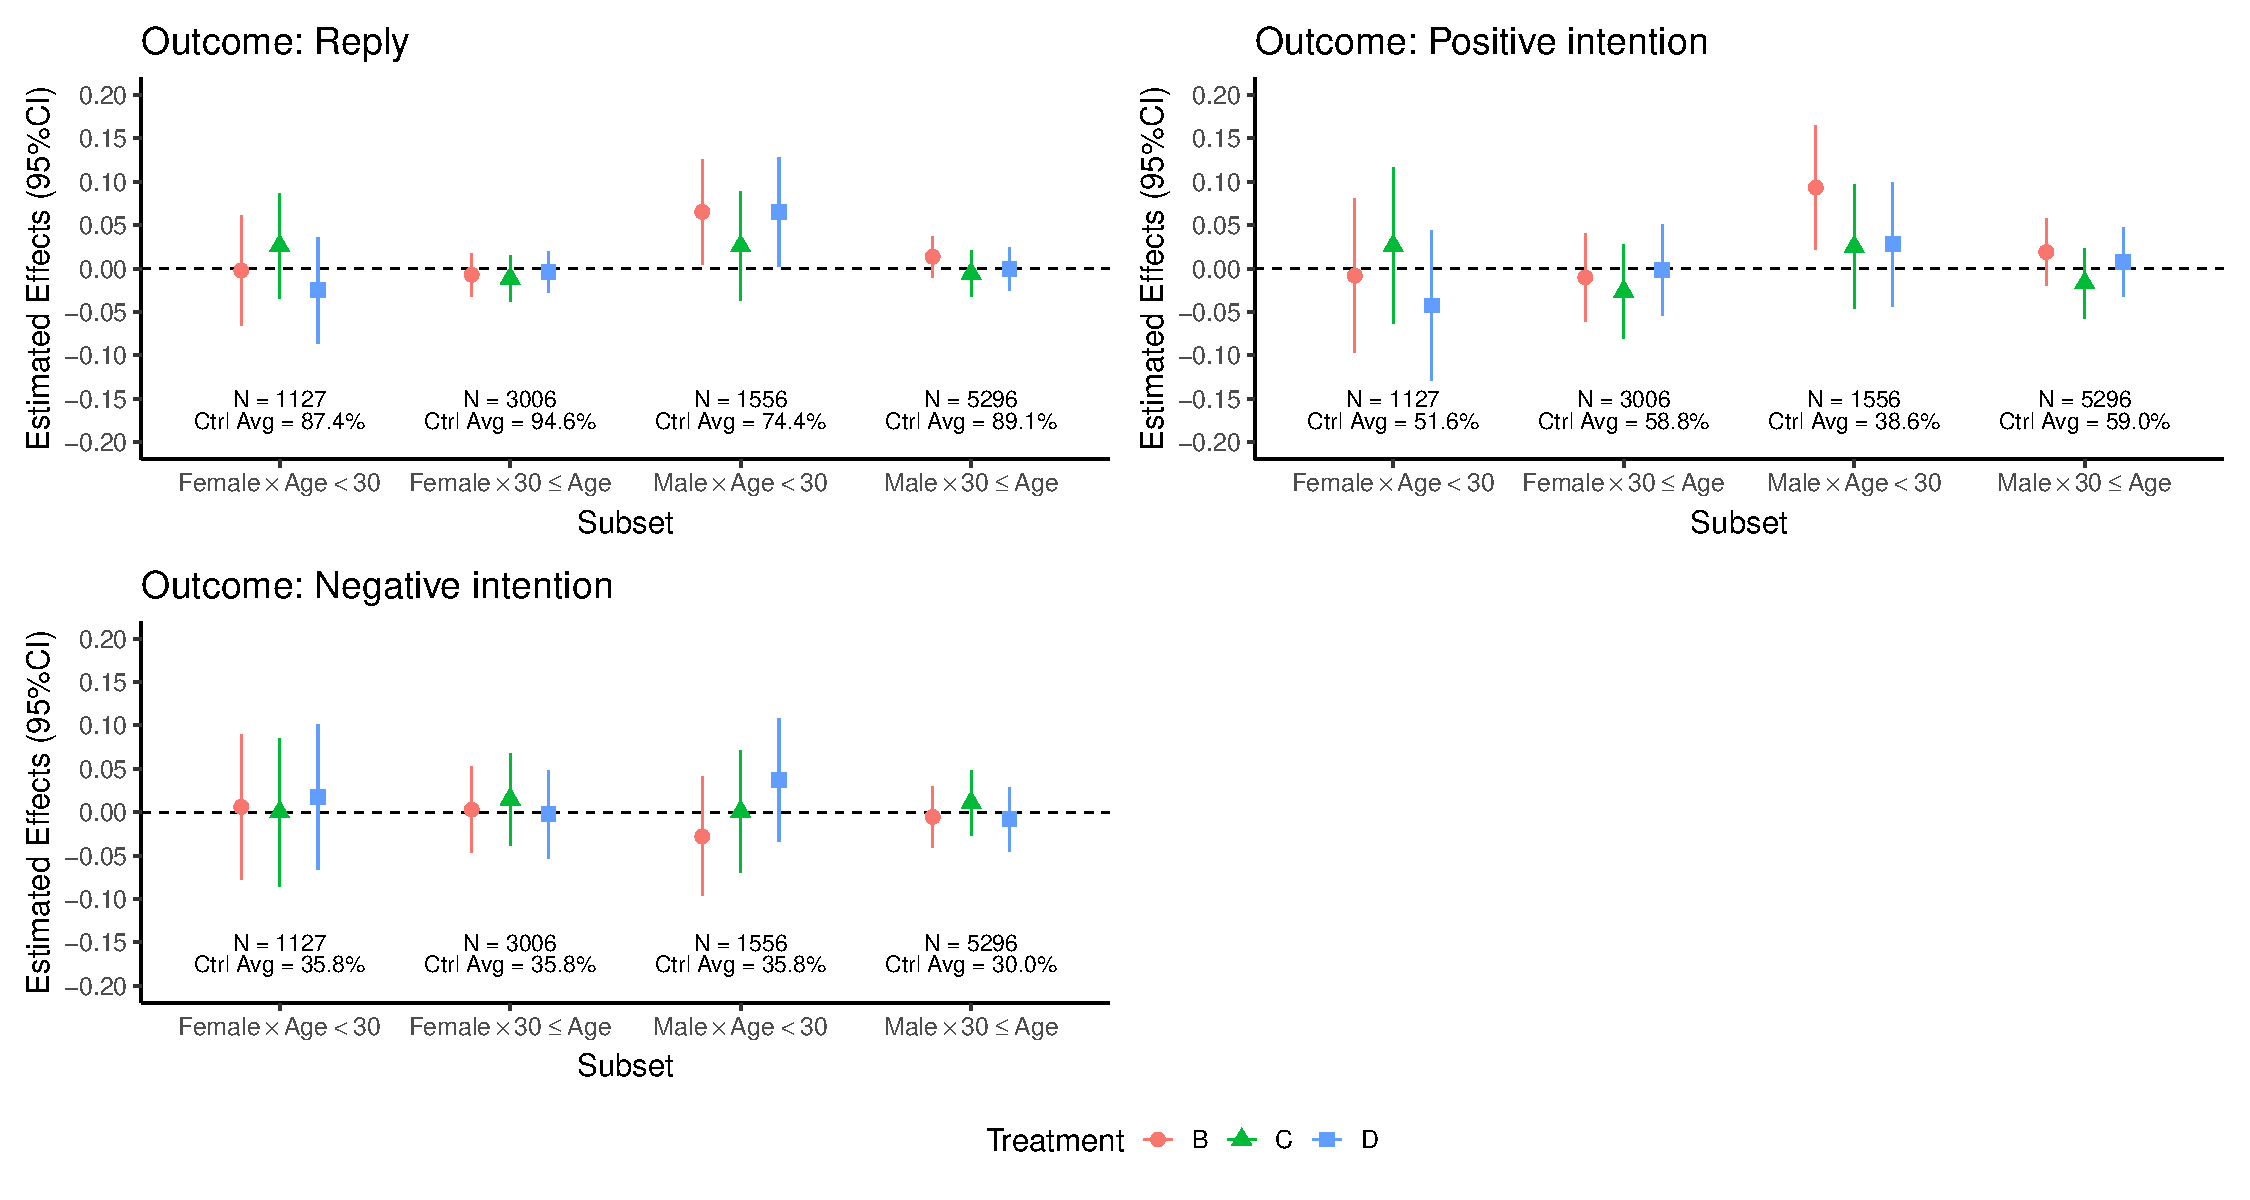
\includegraphics{JMDPRC~2/figure-latex/coefplot-reg-stock-subset-1} \caption{Effect on Reply and Intentions by Gender and Age Group. Notes: These plots show the average effect (and associated 95 percent confidential interval) on each outcome by gender and age group. We use robust standard errors. We control number of past coordinations, number of hospitals per 10 square kilometers, number of hospitals with PBSC collection per 10 square kilometers, number of hospitals with BM collection per 10 square kilometers, month and week dummies.}\label{fig:coefplot-reg-stock-subset}
\end{figure}

Next, to test for heterogeneity in message effects, we divide the sample into four subsets by gender and age (under 30 or not) and estimate the message effects in each subset. Figure \ref{fig:coefplot-reg-stock-subset} presents the coefficient plots. The results show that experimental arms B and D, which include the probability message, increase the response rate of men in their 20s by approximately 6 percentage points (\(8.06\)\% increase, since the control mean is \(74.4\)\%), which is statistically significant at the 5\% level. In particular, experimental arm B, to which only the probability message was added, increased the number of responses with positive intentions by approximately 10 percentage points (\(25.91\)\% increase, because the control mean is \(38.6\)\%), which is also statistically significant. However, for the other gender and age groups, the treatment messages have no statistically significant effect on responses and intentions.

In the control group, approximately 50\% (\(=38.6/74.4\)) of men in their 20s who responded to the compatibility notice were willing to donate, which is lower than the willingness rate of respondents in the other gender and age groups.\footnote{For women in their 20s, 59 (\(=51.6/87.4\))\%; for men over 30, 66 (\(=59.0/89.1\))\%; for women over 30, 62 (\(=58.8/94.6\))\%.} Experimental arm B (probability message) raises the intention rate of male respondents in their 20s from 50\% to 60\% (\(=(38.6 + 10)/(74.4 + 6)\)). In addition, young men have better transplant outcomes than men of other sexes and ages. Taken together, we can say that the probability message improves coordination efficiency in the sense that it encourages behavioral change (initiation of coordination) in desirable donors.

\hypertarget{rcf}{%
\subsection{Random Causal Forest}\label{rcf}}

To further explore the heterogeneity of message effects, we use random causal forests (RCF), which allows us to test the heterogeneous treatment effects in a fully nonparametric manner \citep{Athey2016, Wager2018}. The method is based on a regression tree algorithm and estimates the average treatment effect conditional on the observed characteristics. This method has been used in various contexts, including labor \citep{Davis2017}, education \citep{Carlana2022}, and energy conservation \citep{Murakami2022}.

The algorithm splits the sample into two subsamples (leaves) using one of the covariates \(X_j\). Specifically, the algorithm divides the sample into samples for which \(X_j \le x\) and \(X_j > x\). The regression tree determines a specific threshold \(x\) to minimize the mean squared error of the outcome variable. Given that the RCF aims to estimate the average treatment effect of a leaf (conditional average treatment effect), the threshold \(x\) is set to minimize the expected mean squared error of the predicted treatment effect. This minimization is achieved by increasing the variance in the conditional mean treatment effect across leaves (heterogeneity) and decreasing the variance within leaves. This splitting process is repeated for each leaf until the termination condition is reached. RCF predicts the conditional mean treatment effect on terminal leaves.

A disadvantage of the regression tree algorithm is that the variance in the predictions increases (overfitting), which reduces the accuracy of the predictions. To prevent this, RCF introduces an algorithm called the ensemble method. It creates thousands of subsamples and grows a tree for each subsample. The final result is the average of the predictions from thousands of trees.\footnote{For technical details, see \citet{Athey2016} and \citet{Wager2018}. This study also uses a technique called generalized random forests, which treats RCF as a special case; however, the intuition remains the same. See \citet{Athey2019} and \citet{Athey2019a} for details on generalized random forests.}

RCF predicts the treatment effect from the observed characteristics. In other words, it can predict the treatment effects based on individual characteristics, even for individuals who did not receive the intervention. This method assumes that treatment assignment is conditionally independent of the potential outcome variable. In our study, this method could be used because the experimental arm was approximately randomly assigned. This subsection focuses on the effects on intentions. The covariates used in the RCF are gender, age, past coordination experience, and the density of hospitals in the area of residence.

\begin{figure}[t]
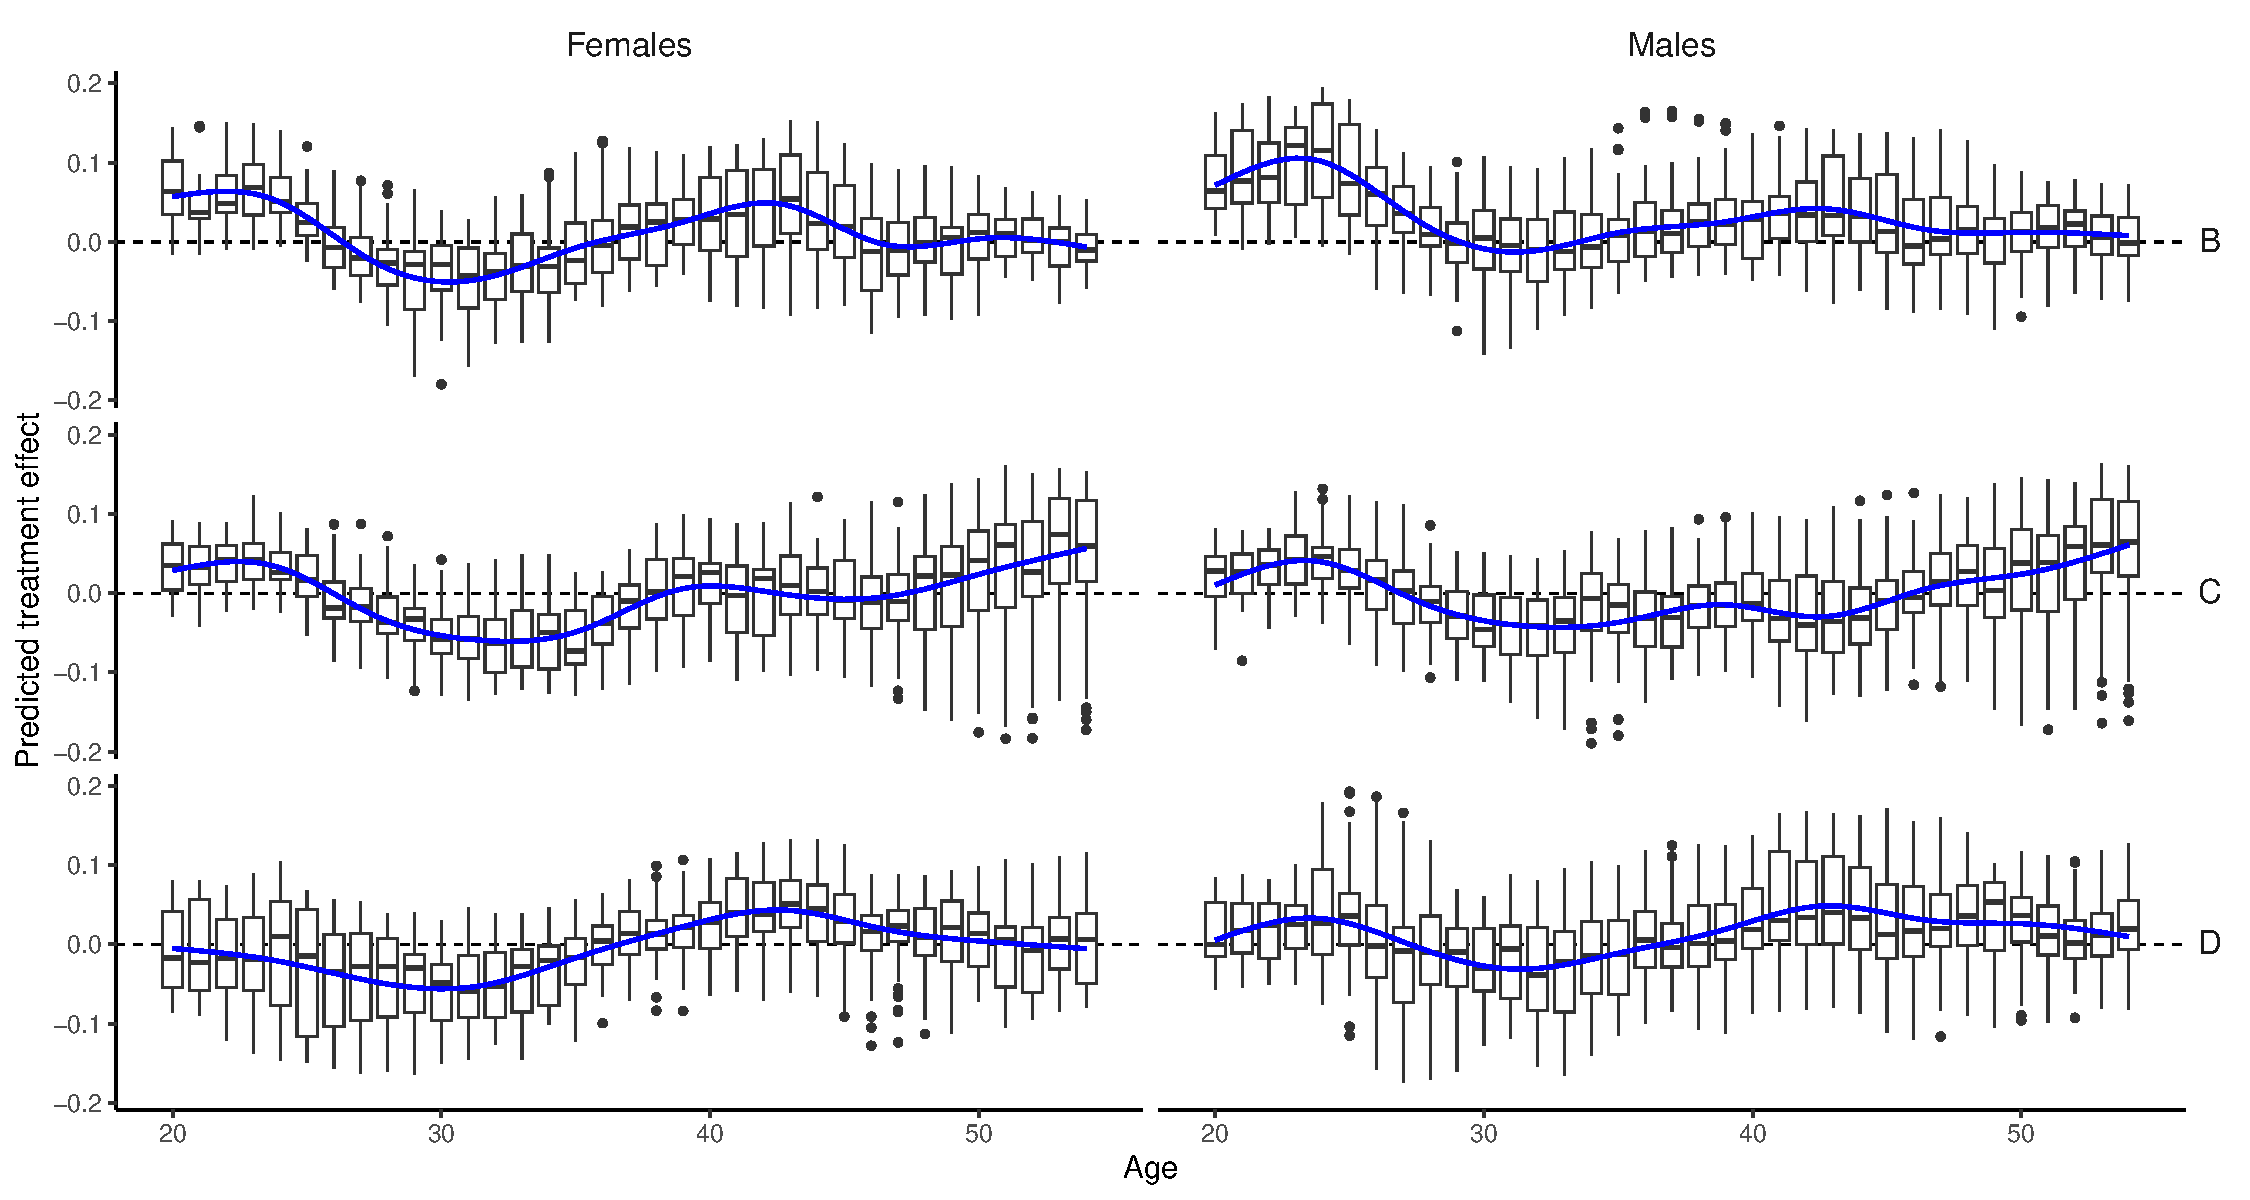
\includegraphics{JMDPRC~2/figure-latex/boxplot-rcf-int-1} \caption{Boxplot of Predicted Treatment Effects by Treatment, Gender and Age. Notes: Fitted line represents GAM smoothing. Covariates are gender, age, number of past coordinations, number of hospitals per 10 square kilometers, number of hospitals with PBSC collection per 10 square kilometers, and number of hospitals with BM collection per 10 square kilometers.}\label{fig:boxplot-rcf-int}
\end{figure}

Figure \ref{fig:boxplot-rcf-int} shows the distribution of the predicted treatment effects for each experimental arm by age. Notably, the effect in experimental arm B is positive for all men under 25 years of age. As a result, the RCF shows that the average effect of experimental arm B for men in their 20s is \(12.1\) percentage points, which is close to the results of the subsample analysis of the linear probability model presented in Figure \ref{fig:coefplot-reg-stock-subset} (see Table \ref{tab:rcf-int-cate} in the Appendix).

For other genders and ages, the message effects are heterogeneous. For example, for some men in their 30s and 40s, the effect of experimental arm B is greater than 10 percentage points. They live in areas with a relatively large number of hospitals and have lower travel costs for coordination and donations (see Table \ref{tab:rcf-middle-male} in the Appendix). Experimental arm C, with only the Early Coordination message added, has a negative effect on most women in their early 30s. For men and women in their late 40s and older, the median effect of experimental arm C is positive, but widely distributed.\footnote{Surprisingly, among men and women in this age group, for whom experimental arm C has a positive effect, live in areas with relatively fewer hospitals (higher traveling costs). See Tables \ref{tab:rcf-older-male} and \ref{tab:rcf-older-female} in the Appendix.}

\begin{table}

\caption{\label{tab:rcf-int-corr}Correlation of Predicted Treatment Effects}
\centering
\fontsize{9}{11}\selectfont
\begin{threeparttable}
\begin{tabular}[t]{lcccccccc}
\toprule
\multicolumn{1}{c}{ } & \multicolumn{8}{c}{Treatment effect of D} \\
\cmidrule(l{3pt}r{3pt}){2-9}
\multicolumn{1}{c}{ } & \multicolumn{2}{c}{Female} & \multicolumn{2}{c}{Male} & \multicolumn{2}{c}{Female} & \multicolumn{2}{c}{Male} \\
\cmidrule(l{3pt}r{3pt}){2-3} \cmidrule(l{3pt}r{3pt}){4-5} \cmidrule(l{3pt}r{3pt}){6-7} \cmidrule(l{3pt}r{3pt}){8-9}
\multicolumn{1}{c}{ } & \multicolumn{1}{c}{Age < 30} & \multicolumn{1}{c}{30 < Age} & \multicolumn{1}{c}{Age < 30} & \multicolumn{1}{c}{30 < Age} & \multicolumn{1}{c}{Age < 30} & \multicolumn{1}{c}{30 < Age} & \multicolumn{1}{c}{Age < 30} & \multicolumn{1}{c}{30 < Age} \\
\cmidrule(l{3pt}r{3pt}){2-2} \cmidrule(l{3pt}r{3pt}){3-3} \cmidrule(l{3pt}r{3pt}){4-4} \cmidrule(l{3pt}r{3pt}){5-5} \cmidrule(l{3pt}r{3pt}){6-6} \cmidrule(l{3pt}r{3pt}){7-7} \cmidrule(l{3pt}r{3pt}){8-8} \cmidrule(l{3pt}r{3pt}){9-9}
  & (1) & (2) & (3) & (4) & (5) & (6) & (7) & (8)\\
\midrule
(Intercept) & \num{-0.037}*** & \num{0.006}*** & \num{-0.017}*** & \num{0.013}*** & \num{-0.034}*** & \num{0.006}*** & \num{0.004}* & \num{0.008}***\\
 & (\num{0.002}) & (\num{0.001}) & (\num{0.002}) & (\num{0.001}) & (\num{0.002}) & (\num{0.001}) & (\num{0.002}) & (\num{0.001})\\
(B + C) & \num{0.290}*** & \num{0.364}*** & \num{0.355}*** & \num{0.425}*** &  &  &  & \\
 & (\num{0.020}) & (\num{0.007}) & (\num{0.019}) & (\num{0.007}) &  &  &  \vphantom{1} & \\
B &  &  &  &  & \num{-0.013} & \num{0.410}*** & \num{-0.070}** & \num{0.655}***\\
 &  &  &  &  & (\num{0.034}) & (\num{0.014}) & (\num{0.028}) & (\num{0.015})\\
C &  &  &  &  & \num{0.677}*** & \num{0.323}*** & \num{0.921}*** & \num{0.272}***\\
 &  &  &  &  & (\num{0.038}) & (\num{0.013}) & (\num{0.033}) & (\num{0.011})\\
\addlinespace[0.3em]
\multicolumn{9}{l}{\textit{Linear combination test (F-test)}}\\
\hspace{1em}(B + C) - 1 & \num{-0.710}*** & \num{-0.636}*** & \num{-0.645}*** & \num{-0.575}*** &  &  &  & \\
\hspace{1em} & (\num{0.020}) & (\num{0.007}) & (\num{0.019}) & (\num{0.007}) &  &  &  & \\
\hspace{1em}B - C &  &  &  &  & \num{-0.690}*** & \num{0.087}*** & \num{-0.991}*** & \num{0.383}***\\
\hspace{1em} &  &  &  &  & (\num{0.062}) & (\num{0.022}) & (\num{0.050}) & (\num{0.022})\\
\midrule
Num.Obs. & \num{1132} & \num{3018} & \num{1566} & \num{5333} & \num{1132} & \num{3018} & \num{1566} & \num{5333}\\
\bottomrule
\end{tabular}
\begin{tablenotes}
\item Notes: * p < 0.1, ** p < 0.05, *** p < 0.01. The robust standard errors are in parentheses. 
\end{tablenotes}
\end{threeparttable}
\end{table}

In addition to examining heterogeneity, we discuss the mechanism of experimental arm D using the treatment effects predicted by the RCF. To test the effects of the cognitive load due to information overload, experimental arm D adds both a probability message (experimental arm B) and an early coordination message (experimental arm C).

If the matched donor fully understands the information in experimental arm D, its effect should be the sum of the effects of experimental arms B and C. To test this point, columns (1)--(4) of Table \ref{tab:rcf-int-corr} regress the predicted treatment effect of experimental arm D on the sum of the predicted effects of experimental arms B and C. For each gender and age group, a 1-point increase in the sum of the effects of experimental arms B and C increases the effect of experimental arm D by \(0.3\)--\(0.4\) points. As we can reject the null hypothesis that the coefficient of the sum of the predicted effects of experimental arms B and C is 1 (the sum of their predicted effects is equal to the effect of experimental arm D), this suggests that the matched donors do not fully understand the information in experimental arm D and are cognitively overloaded because of information overload.

A matched donor who does not completely receive information would value either the probability message or the early coordination message or would discount the two pieces of information equally. To test this point, columns (5)--(8) of Table \ref{tab:rcf-int-corr} regress the predicted treatment effects of experimental arm D on those of experimental arms B and C. The results show that for men and women in their 20s, the partial correlations between experimental arms C and D are stronger than those between experimental arms B and D, which is a statistically significant difference according to the F-test. This implies that they value the early coordination message more than the probability message. Thus, experimental arm D is ineffective for men in their 20s.

Interestingly, for men and women over 30 years, the partial correlations between experimental arms C and D are weaker than those between experimental arms B and D, which is a statistically significant difference according to the F-test. In other words, they value the probability message more than the early coordination message. Thus, while the median effect of experimental arm C for men and women in their late 40s and older is approximately 8 points, the median treatment effect of experimental arm D is almost zero.

\hypertarget{reply-speed}{%
\subsection{Response Speed to Notification}\label{reply-speed}}

\begin{figure}[t]
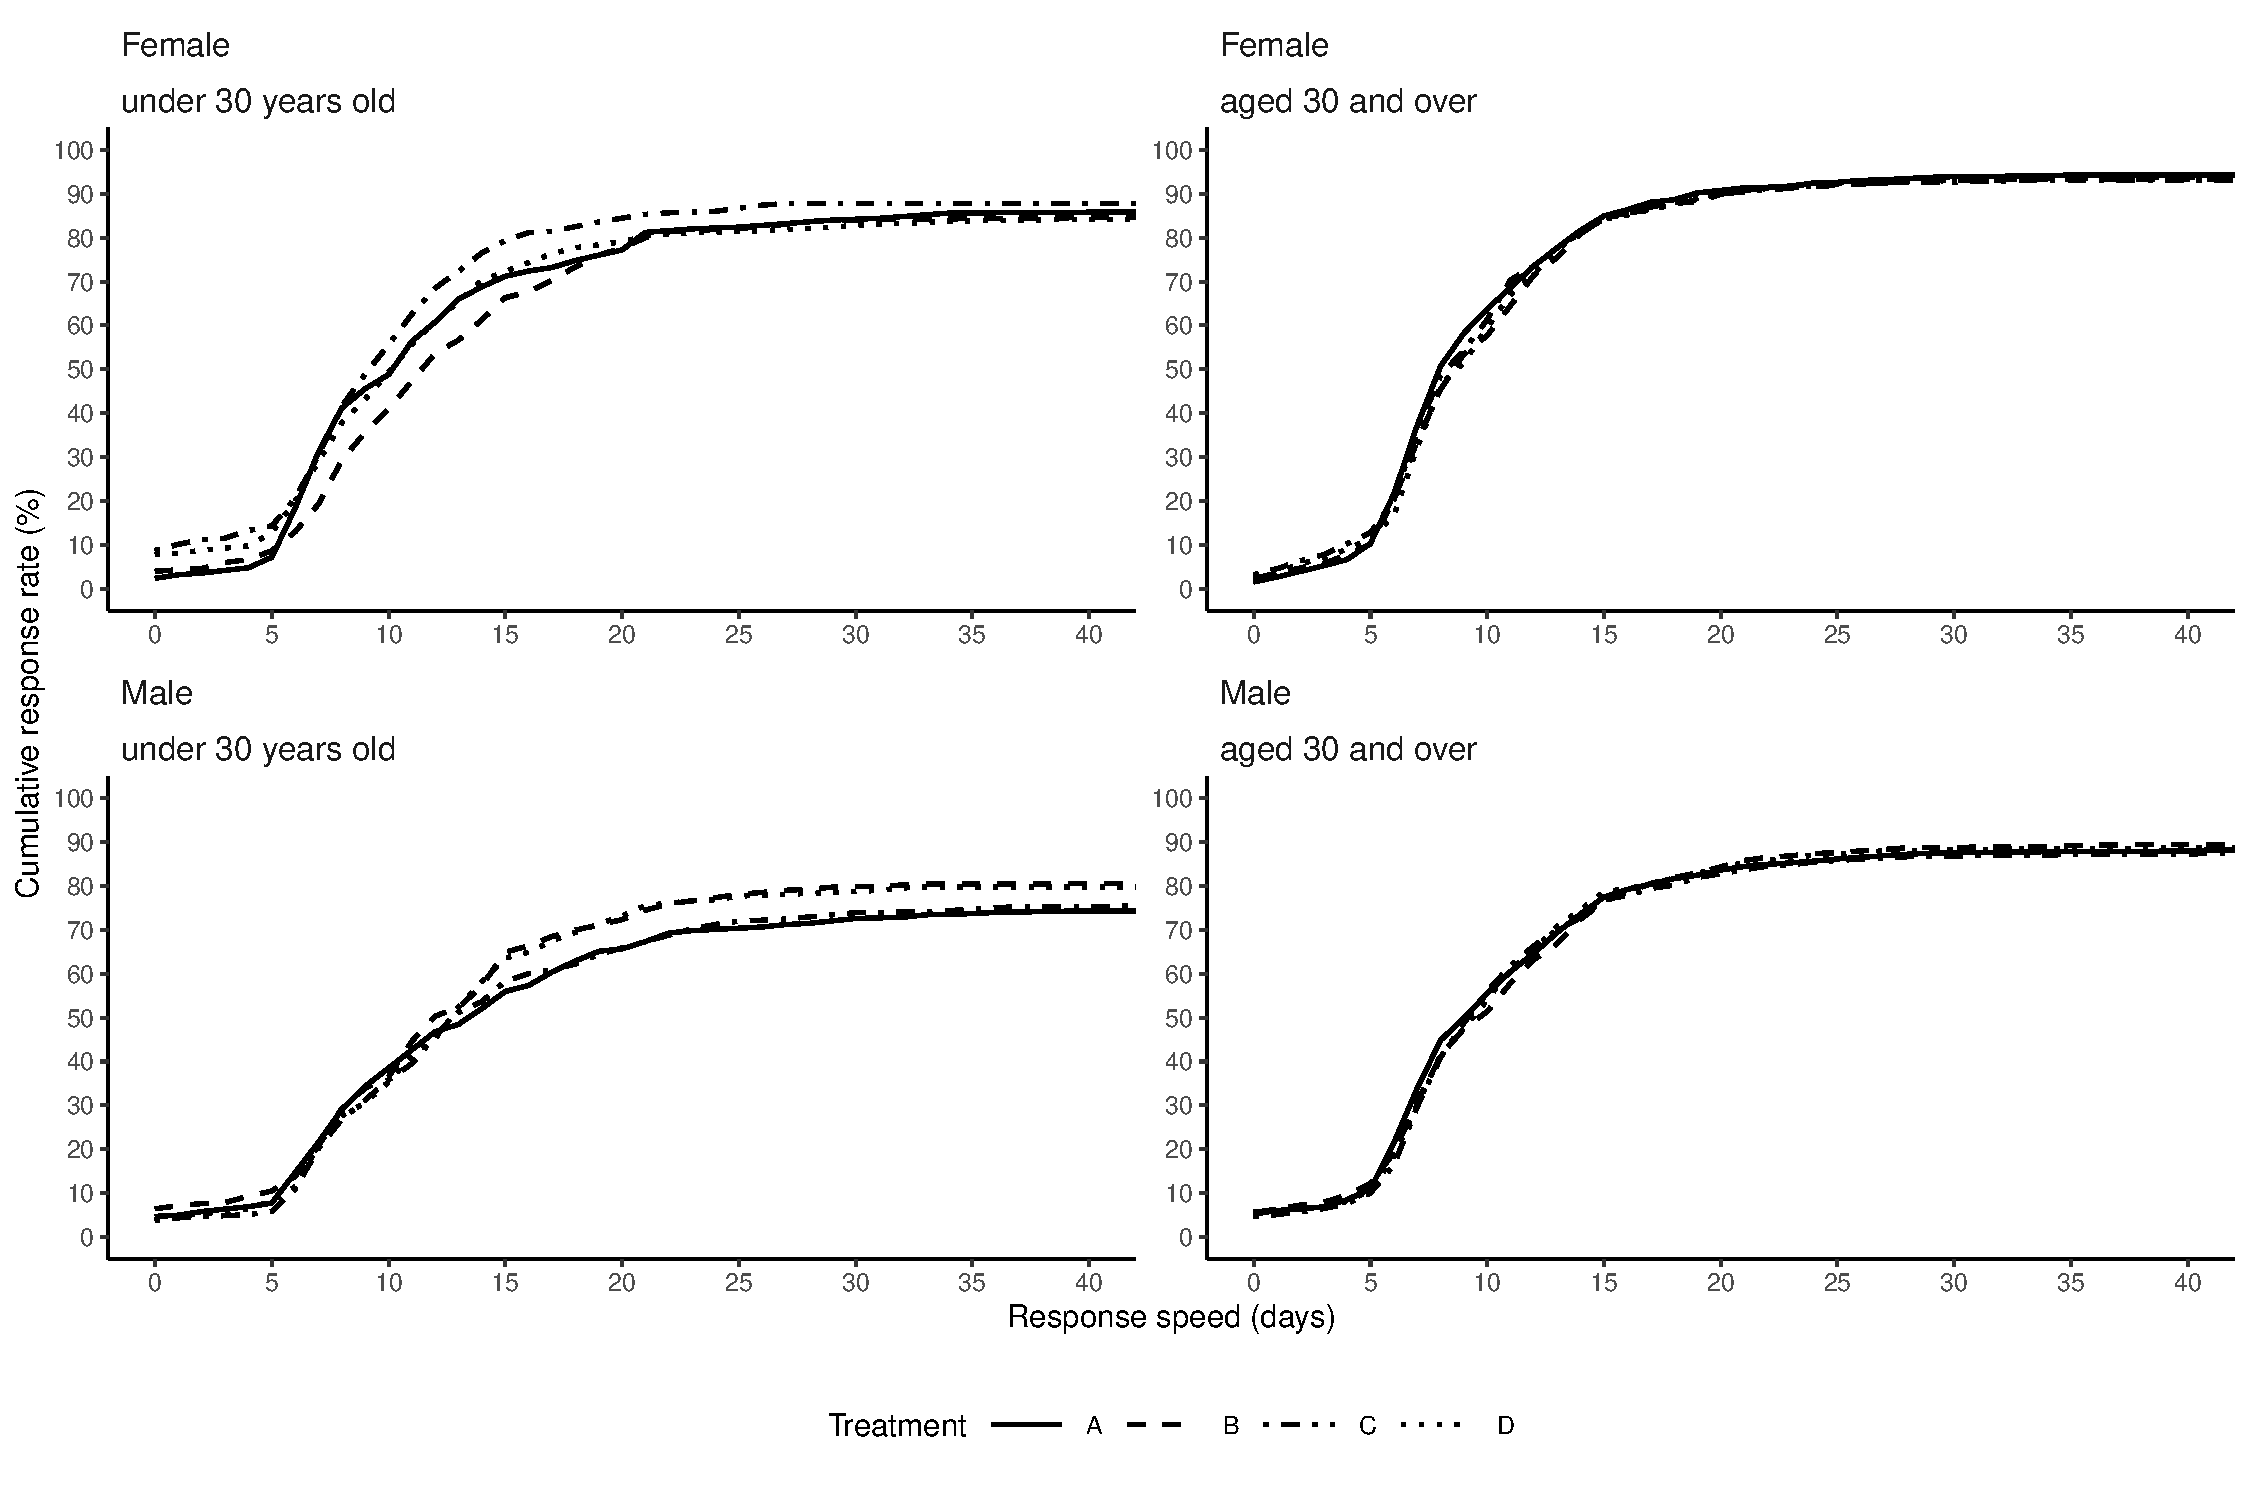
\includegraphics{JMDPRC~2/figure-latex/cumulative-response-rate-1} \caption{Cumulative Response Rates by Gender and Age Group.}\label{fig:cumulative-response-rate}
\end{figure}

The early coordination message states that early coordination increases the patient's transplantation rate. Therefore, this message may encourage early responses to compatibility notice. Figure \ref{fig:cumulative-response-rate} shows the cumulative response rate for the 40 days after the compatibility notice was sent. Given that the effect on responses is heterogeneous by gender and age, as shown in the previous results, we also split the subsample by gender and age and focus on the heterogeneity of the effect on quick responses.

\begin{figure}[t]
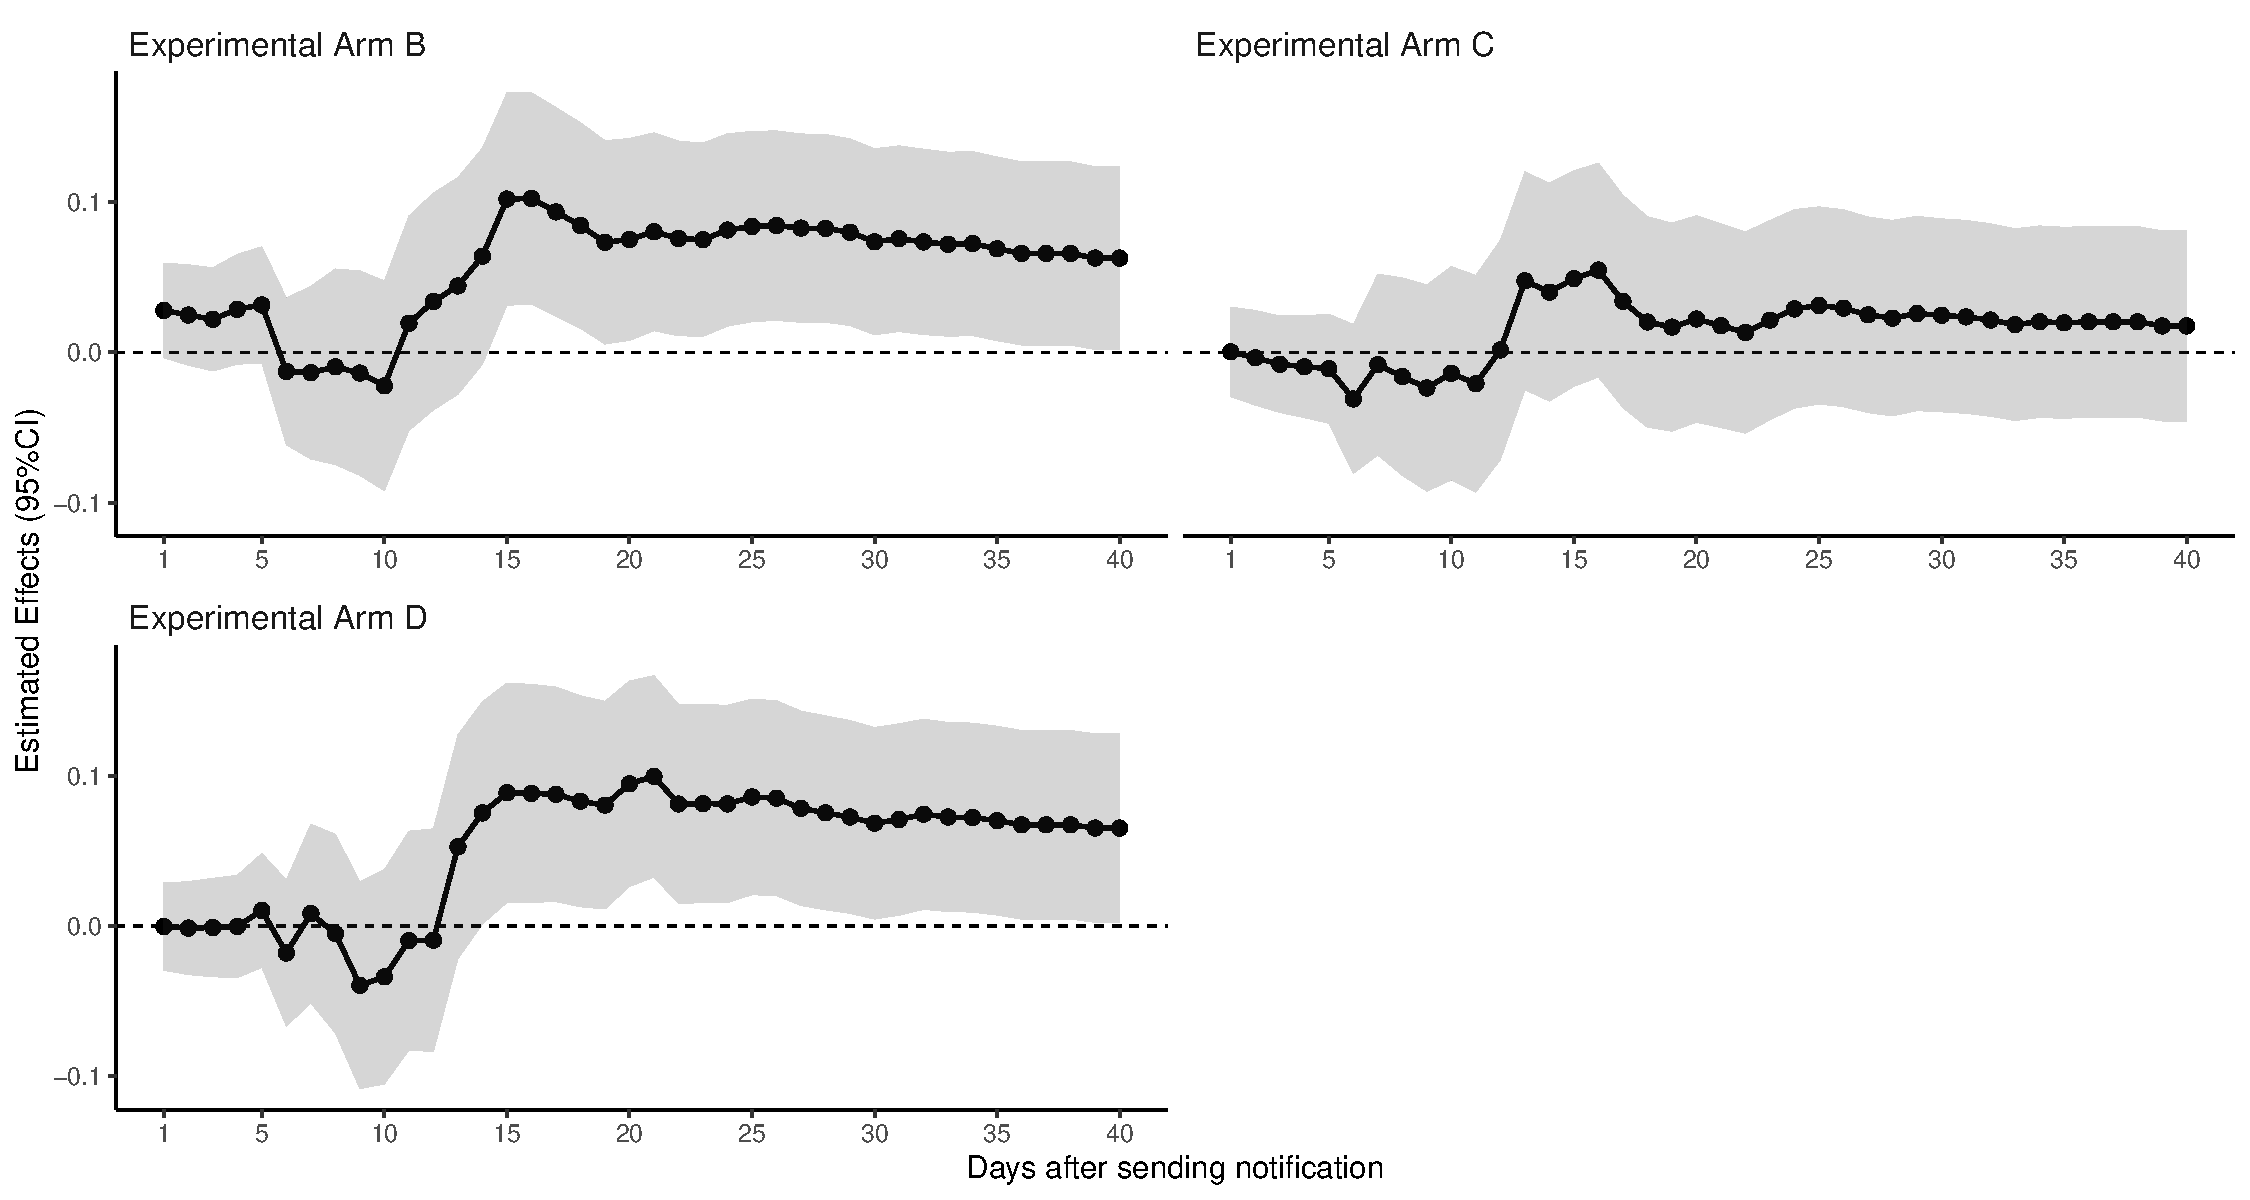
\includegraphics{JMDPRC~2/figure-latex/young-male-flow-1} \caption{Effect on Reply within Specific Days after Sending Notification among Males Less than 30. Notes: These plots show the average effect (and associated 95 percent confidential interval) on cumulative responses on specific days. We use robust standard errors. We control number of past coordinations, number of hospitals per 10 square kilometers, number of hospitals with PBSC collection per 10 square kilometers, number of hospitals with BM collection per 10 square kilometers, month dummies, and week dummies.}\label{fig:young-male-flow}
\end{figure}

While there are no significant differences in the pattern of cumulative response rates for men and women over 30 years, there are some notable results for men and women under 30 years.\footnote{For men and women over 30 years of age, the cumulative response rate for each day differs little between the experimental arms, except for certain periods, and is not statistically significant. See Figure \ref{fig:old-male-flow} and \ref{fig:old-female-flow} in Appendix.} In the group of men in their 20s, 15 days after the compatibility notice was sent, the responses of experimental arms B and D began to increase relative to those of the controls. Consequently, the cumulative response rate of the two experimental arms is statistically significantly higher than that of the control arm (Figure \ref{fig:young-male-flow}).\footnote{In the regression analysis, we created a dummy variable that takes 1 if the potential donor responded within \(d\) days as the outcome variable. If the potential donor responded after \(d\) days or did not respond, the outcome variable is 0.} Given that the compatibility notice recommends a response within 7 days, a response 15 days after the mailing of the compatibility notice cannot be considered an early response. Thus, although experimental arms B and D increased the ultimate response rate among men in their 20s, they did not encourage early responses. This result is natural because the probability message, the intervention in experimental arms B and D, is not intended to encourage early responses. In addition, the trend in experimental arm C, where only Early Coordination messages are added, is almost the same as that in the control, so it cannot be said that Early Coordination messages encourage early responses in this group.

\begin{figure}[t]
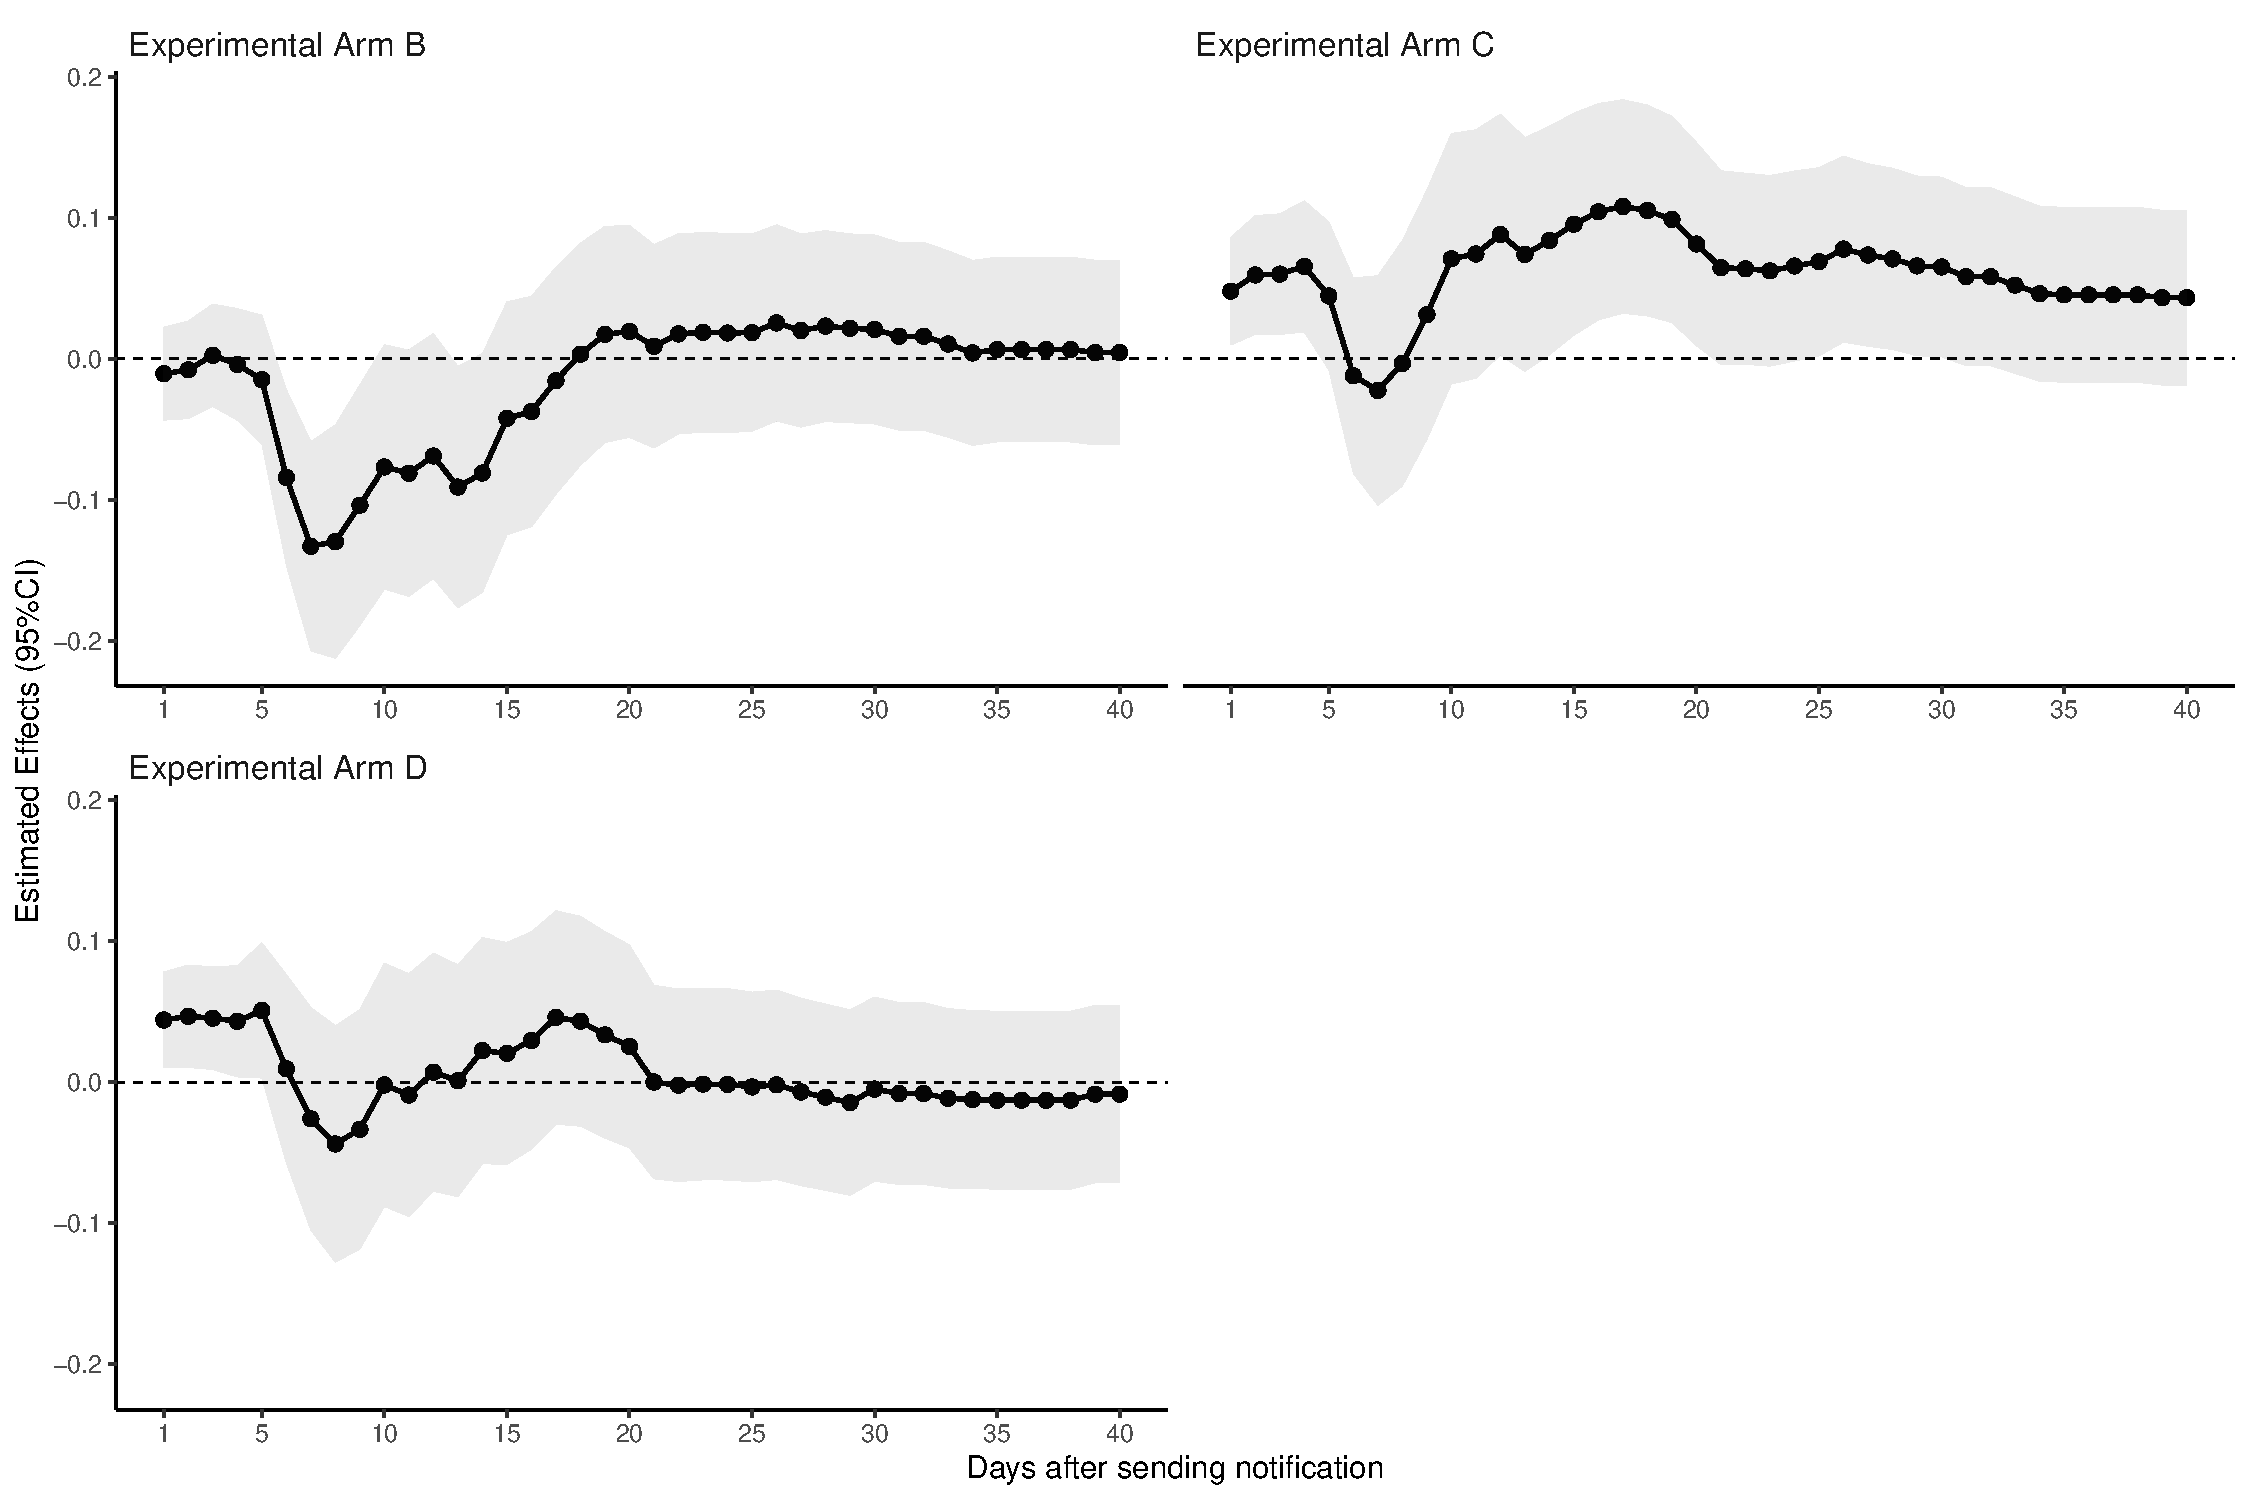
\includegraphics{JMDPRC~2/figure-latex/young-female-flow-1} \caption{Effect on Reply within Specific Days after Sending Notification among Females Less than 30. Notes: These plots show the average effect (and associated 95 percent confidential interval) on cumulative responses on specific days. We use robust standard errors. We control number of past coordinations, number of hospitals per 10 square kilometers, number of hospitals with PBSC collection per 10 square kilometers, number of hospitals with BM collection per 10 square kilometers, month dummies, and week dummies.}\label{fig:young-female-flow}
\end{figure}

In the 20s women group, the responses of experimental arms C and D, with the addition of the early coordination message, increased compared with the control within four days of sending the compatibility message. As a result, the cumulative response rates of the two experimental arms are statistically significantly higher than that of the control arm (Figure \ref{fig:young-female-flow}). In addition, 10 days after the compatibility notice is sent, the responses of experimental arm C begin to temporarily increase relative to the control, but eventually cease to be significantly different from the cumulative response rate of the control. These results suggest that early coordination messages encourage females in their 20s to respond quickly.\footnote{We decompose the effect of message C on responses within four days (early responses) into two parts in terms of intentions and find that it increases positive and negative intentions to the same extent.}

\hypertarget{process}{%
\subsection{Effects on the Coordination Process}\label{process}}

Finally, we examine the impact of messages on each step of the coordination process. As explained in Section \ref{background}, the coordination process comprises four stages: confirmatory typing, candidate selection, final consent, and collection. As the outcome variable, we use a dummy variable that takes the value of 1 if a matched donor has reached each stage.

As in the analysis in Section \ref{intention}, we exclude samples in which coordination appears to have been interrupted, independent of the matched donor willingness. When estimating the effect of confirmatory typing, we exclude cases of interruption due to patient-related reasons. Given that the patient's physician is likely to select a healthier matched donor at the time of candidate selection, cases of interruption of donor health reasons after candidate selection are considered to have occurred independently of the donor's willingness. Thus, when estimating the effects on candidate selection, final consent, and donation, we exclude samples interrupted for patient and samples interrupted for donor health reasons after candidate selection. Note that we should be cautious in our interpretation, because sample exclusion alone may not completely eliminate physician decision-making. In the control group, 24\% of eligible donors underwent confirmatory testing, 8\% became candidates, and 6\% ultimately donated.

\begin{table}

\caption{\label{tab:est-full-coordination}Linear Probability Model of Coordination}
\centering
\fontsize{9}{11}\selectfont
\begin{threeparttable}
\begin{tabular}[t]{lcccccccc}
\toprule
\multicolumn{1}{c}{ } & \multicolumn{2}{c}{CT} & \multicolumn{2}{c}{Candidate} & \multicolumn{2}{c}{Consent} & \multicolumn{2}{c}{Donation} \\
\cmidrule(l{3pt}r{3pt}){2-3} \cmidrule(l{3pt}r{3pt}){4-5} \cmidrule(l{3pt}r{3pt}){6-7} \cmidrule(l{3pt}r{3pt}){8-9}
  & (1) & (2) & (3) & (4) & (5) & (6) & (7) & (8)\\
\midrule
Treatment B & \num{0.033}*** & \num{0.033}*** & \num{0.005} & \num{0.003} & \num{0.006} & \num{0.004} & \num{0.004} & \num{0.002}\\
 & (\num{0.012}) & (\num{0.012}) & (\num{0.008}) & (\num{0.008}) & (\num{0.008}) & (\num{0.008}) & (\num{0.007}) & (\num{0.007})\\
Treatment C & \num{0.015} & \num{0.014} & \num{0.001} & \num{-0.002} & \num{0.002} & \num{-0.001} & \num{0.002} & \num{-0.002}\\
 & (\num{0.012}) & (\num{0.013}) & (\num{0.008}) & (\num{0.009}) & (\num{0.008}) & (\num{0.008}) & (\num{0.007}) & (\num{0.008})\\
Treatment D & \num{0.026}** & \num{0.030}** & \num{0.008} & \num{0.009} & \num{0.010} & \num{0.010} & \num{0.003} & \num{0.003}\\
 & (\num{0.012}) & (\num{0.012}) & (\num{0.009}) & (\num{0.009}) & (\num{0.008}) & (\num{0.008}) & (\num{0.007}) & (\num{0.008})\\
\midrule
Control average & 0.2350 & 0.2350 & 0.0779 & 0.0779 & 0.0687 & 0.0687 & 0.0574 & 0.0574\\
Covariates &  & X &  & X &  & X &  & X\\
Num.Obs. & \num{10435} & \num{10435} & \num{8587} & \num{8587} & \num{8558} & \num{8558} & \num{8441} & \num{8441}\\
\bottomrule
\end{tabular}
\begin{tablenotes}
\item Notes: * p < 0.1, ** p < 0.05, *** p < 0.01. The robust standard errors are in parentheses. Covariates are gender, (demeaned) age, its squared term, number of past coordinations, number of hospitals per 10 square kilometers, number of hospitals with PBSC collection per 10 square kilometers, number of hospitals with BM collection per 10 square kilometers, month dummies, and week dummies.
\end{tablenotes}
\end{threeparttable}
\end{table}

Table \ref{tab:est-full-coordination} lists the results of the full-sample estimation. The results show that experimental arms B and D, which include probability messages, increase the rate of confirmatory typing by approximately 3 percentage points, which is a statistically significant effect. This effect is greater than that of the responses. This is because the likelihood of coordination interruption for donor reasons, including health reasons, is lower in experimental arms B and D than in the control group. Thus, although experimental arms B and D do not increase the overall number of people willing to donate, they maintain their intention to donate, which contributes to a reduction in coordination dropouts.

The effect of experimental arms B and D on the stage after candidate selection is less than 1 percentage point and not statistically significant. These findings should be interpreted with caution. Given that our intervention did not affect demand (number of patients), if our intervention had increased the number of people who reached confirmatory typing, it should have increased the number of people who were not selected as candidates for exogenous reasons.

In experimental arm B and the control group, the numbers of potential donors who reached confirmatory typing were 774 and 564, respectively. Therefore, experimental arm B would have increased the number of confirmatory typings by 210. The number of potential donors who were not selected as candidates for patient or donor health reasons was 556 in the experimental arm B and 385 in the control group. This means that experimental arm B has 171 more people who were not selected as candidates for exogenous reasons. Thus, the estimates include not only the effect of our intervention but also the effect of the demand for stem cell transplants.

\begin{figure}[t]
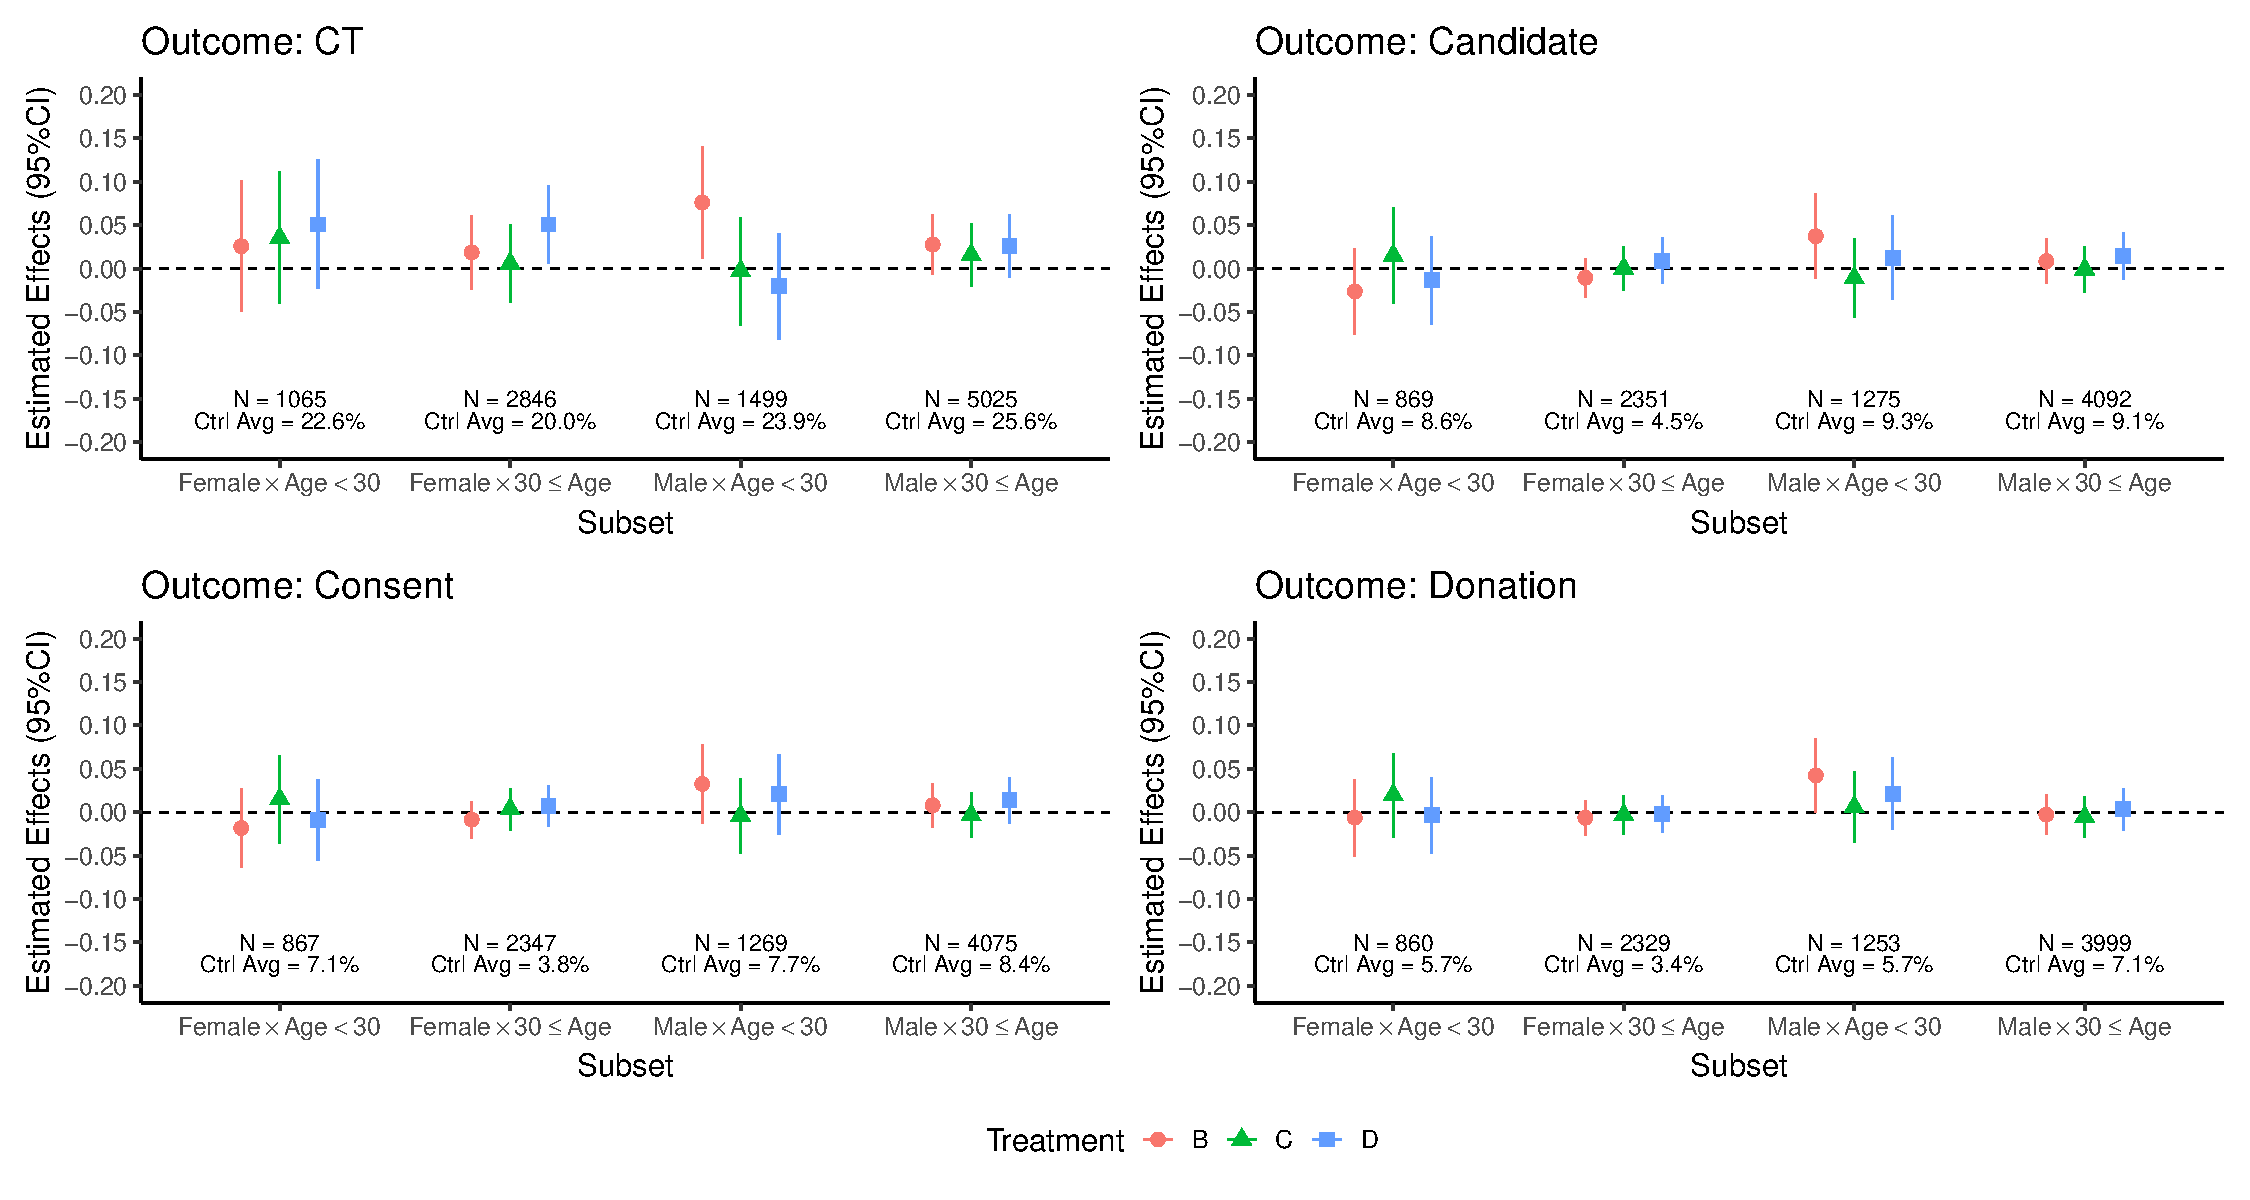
\includegraphics{JMDPRC~2/figure-latex/coefplot-reg-subsample-coordination-1} \caption{Effect on Coordination by Gender and Age Group. Note: These plots show the average effect (and associated 95 percent confidential interval) on each outcome by gender and age group. We use robust standard errors. We control number of past coordinations, number of hospitals per 10 square kilometers, number of hospitals with PBSC collection per 10 square kilometers, number of hospitals with BM collection per 10 square kilometers, month dummies, and week dummies.}\label{fig:coefplot-reg-subsample-coordination}
\end{figure}

Figure \ref{fig:coefplot-reg-subsample-coordination} divides the sample into four subsets by gender and age (under 30 or not) and estimates the message effect in each subset. The results show that experimental arm B increases the proportion of men in their 20s who reach confirmatory typing by approximately 8 percentage points, which is statistically significant. Thus, it is possible that experimental arm B not only increases the willingness of men in their 20s to donate but also maintains it.

Experimental arm B may increase donations among men in their 20s by 4 percentage points, which is statistically significant at the 10\% level. However, the effect on candidate selection and final consent is not statistically significant. As noted earlier, this effect may reflect not only the effect of our intervention but also the demand for stem cell transplants. If younger males have better transplant outcomes, the demand for stem cell transplants may be higher in this generation than in other genders and ages. The effect on donations may include a demand effect. In addition, experimental arm C, which encouraged early responses from women in their 20s, had no statistically significant effect on the coordination of this generation.

\hypertarget{conclusion}{%
\section{Discussion and Conclusions}\label{conclusion}}

This study examined the effects of providing information to increase the willingness to donate among potential donors enrolled in the JMDP. The results showed that information about a low number of HLA-matched donors per patient (probability message) increased the willingness to donate among men in their 20s by approximately 10 percentage points. However, when we simultaneously provide the information that early coordination increases a patient's transplant rate (early coordination message), the positive effect of the probability message disappears because they give more weight to the early coordination message in their decision-making. In addition, this message increased the rate of achieving confirmatory typing by approximately 8 percentage points and may increase the transplant rate by 5 percentage points. In terms of numbers, the Probability message increased the number of transplanted donors from 71 to 121. Thus, information about HLA matching of others would increase the efficiency of coordination in the sense that the message encourages donors with good transplant performance to proceed with coordination.

These results suggest that men in their 20s overestimate the number of HLA-matched donors and engage in free-riding behavior. There are two possible reasons for the statistically insignificant effect of the probability message on the other genders and ages. First, compared to men in their 20s, others may have correctly estimated the number of HLA-matched donors. In this case, the probability message should not affect the decisions of potential donors.

The second possibility is that the altruistic preferences of men in their 20s differ from those of other genders and age groups. Economic studies suggest that there are two main types of motives for altruistic behavior: warm glow, in which one gains utility from one's altruistic behavior; and pure altruism, in which one gains utility from the results of altruistic behavior, such as the production of public goods \citep{Andreoni1990}. Those with relatively stronger warm glow were less likely to engage in free-riding behavior because they were less concerned about the actions of others. Thus, compared to men in their 20s, others may have a warm glow preference as the main driver of altruistic behavior. In short, the heterogeneity in probability messages can be explained by differences in beliefs or motivations.

The early coordination message had no effect on the overall response rate among women in their 20s, but had a positive effect on shorter responses (4 days or less). This suggests that it shortens the timing of replies rather than encouraging response behavior itself. Owing to our data limitations, we cannot test whether this message shortens the time to transplantation for patients; however, the information might contribute to a shorter coordination period.

The lack of effect for other genders and ages may be due to the possibility that others already have this information. Alternatively, women in their 20s may have a stronger degree of present bias and a greater tendency toward delayed behavior than other generations. The heterogeneity of the message effect could be explained by differences in information possession or time preferences.

Although this study identifies the causal effects of information provision through field experiments, it is limited by the fact that the data and experimental design do not allow for the identification of the mechanisms described above, which may be an issue for future work. This study has several practical implications. As discussed in Section \ref{intro}, maintaining the intention of potential donors is a challenge for bone marrow donor programs due to the time lag between intention and behavior. In particular, young donors with good transplant outcomes are likely to fail to maintain their intentions and drop out of the program. This study suggests that information provided by the bone marrow donor program office at the time of matching with a patient may promote behavioral changes in young potential donors and may be one measure to address this problem. However, some studies \citep[for example,][]{Switzer2018} have shown that information provision is ineffective, so it is expected that the effectiveness of our information provision will be tested in bone marrow donor programs in other countries.

\clearpage

\hypertarget{appendix}{%
\section*{Appendix}\label{appendix}}
\addcontentsline{toc}{section}{Appendix}

\begin{table}[H]

\caption{\label{tab:logit-stock}Logit Model of Reply and Intention}
\centering
\fontsize{9}{11}\selectfont
\begin{threeparttable}
\begin{tabular}[t]{lcccccc}
\toprule
\multicolumn{3}{c}{ } & \multicolumn{4}{c}{Intention} \\
\cmidrule(l{3pt}r{3pt}){4-7}
\multicolumn{1}{c}{ } & \multicolumn{2}{c}{Reply} & \multicolumn{2}{c}{Positive} & \multicolumn{2}{c}{Negative} \\
\cmidrule(l{3pt}r{3pt}){2-3} \cmidrule(l{3pt}r{3pt}){4-5} \cmidrule(l{3pt}r{3pt}){6-7}
  & (1) & (2) & (3) & (4) & (5) & (6)\\
\midrule
Treatment B & \num{1.11} & \num{1.15} & \num{1.09} & \num{1.09} & \num{0.95} & \num{0.97}\\
 & {}[\num{0.94}, \num{1.31}] & {}[\num{0.96}, \num{1.37}] & {}[\num{0.98}, \num{1.22}] & {}[\num{0.98}, \num{1.22}] & {}[\num{0.85}, \num{1.06}] & {}[\num{0.86}, \num{1.09}]\\
Treatment C & \num{0.95} & \num{1.02} & \num{0.98} & \num{0.99} & \num{1.00} & \num{1.03}\\
 & {}[\num{0.80}, \num{1.12}] & {}[\num{0.86}, \num{1.22}] & {}[\num{0.88}, \num{1.09}] & {}[\num{0.88}, \num{1.11}] & {}[\num{0.89}, \num{1.12}] & {}[\num{0.91}, \num{1.16}]\\
Treatment D & \num{1.06} & \num{1.06} & \num{1.02} & \num{1.02} & \num{1.01} & \num{1.00}\\
 & {}[\num{0.89}, \num{1.26}] & {}[\num{0.89}, \num{1.27}] & {}[\num{0.91}, \num{1.14}] & {}[\num{0.91}, \num{1.15}] & {}[\num{0.90}, \num{1.13}] & {}[\num{0.89}, \num{1.13}]\\
\midrule
Covariates &  & X &  & X &  & X\\
Num.Obs. & \num{10985} & \num{10985} & \num{10985} & \num{10985} & \num{10985} & \num{10985}\\
Log.Lik. & \num{-3884.517} & \num{-3712.289} & \num{-7534.803} & \num{-7364.638} & \num{-6945.023} & \num{-6869.968}\\
\bottomrule
\end{tabular}
\begin{tablenotes}
\item Notes: We show odds ratios and associated 95 percent confidential intervals in square brackets. Covariates are gender, (demeaned) age, its squared term, number of past coordinations, number of hospitals per 10 square kilometers, number of hospitals with PBSC collection per 10 square kilometers, number of hospitals with BM collection per 10 square kilometers, month dummies, and week dummies.
\end{tablenotes}
\end{threeparttable}
\end{table}

\begin{table}[H]

\caption{\label{tab:logit-coordination}Logit Model of Coordination}
\centering
\fontsize{9}{11}\selectfont
\begin{threeparttable}
\begin{tabular}[t]{lcccccccc}
\toprule
\multicolumn{1}{c}{ } & \multicolumn{2}{c}{CT} & \multicolumn{2}{c}{Candidate} & \multicolumn{2}{c}{Consent} & \multicolumn{2}{c}{Donation} \\
\cmidrule(l{3pt}r{3pt}){2-3} \cmidrule(l{3pt}r{3pt}){4-5} \cmidrule(l{3pt}r{3pt}){6-7} \cmidrule(l{3pt}r{3pt}){8-9}
  & (1) & (2) & (3) & (4) & (5) & (6) & (7) & (8)\\
\midrule
Treatment B & \num{1.19} & \num{1.20} & \num{1.07} & \num{1.04} & \num{1.09} & \num{1.06} & \num{1.07} & \num{1.04}\\
 & {}[\num{1.05}, \num{1.35}] & {}[\num{1.05}, \num{1.36}] & {}[\num{0.86}, \num{1.33}] & {}[\num{0.83}, \num{1.31}] & {}[\num{0.87}, \num{1.38}] & {}[\num{0.83}, \num{1.35}] & {}[\num{0.83}, \num{1.39}] & {}[\num{0.80}, \num{1.35}]\\
Treatment C & \num{1.08} & \num{1.08} & \num{1.01} & \num{0.97} & \num{1.04} & \num{0.99} & \num{1.03} & \num{0.98}\\
 & {}[\num{0.95}, \num{1.23}] & {}[\num{0.94}, \num{1.24}] & {}[\num{0.81}, \num{1.27}] & {}[\num{0.76}, \num{1.23}] & {}[\num{0.82}, \num{1.32}] & {}[\num{0.77}, \num{1.27}] & {}[\num{0.79}, \num{1.34}] & {}[\num{0.74}, \num{1.29}]\\
Treatment D & \num{1.15} & \num{1.18} & \num{1.12} & \num{1.12} & \num{1.16} & \num{1.16} & \num{1.06} & \num{1.05}\\
 & {}[\num{1.01}, \num{1.31}] & {}[\num{1.03}, \num{1.35}] & {}[\num{0.90}, \num{1.40}] & {}[\num{0.89}, \num{1.41}] & {}[\num{0.92}, \num{1.46}] & {}[\num{0.91}, \num{1.47}] & {}[\num{0.81}, \num{1.37}] & {}[\num{0.80}, \num{1.38}]\\
\midrule
Covariates &  & X &  & X &  & X &  & X\\
Num.Obs. & \num{10435} & \num{10435} & \num{8587} & \num{8587} & \num{8558} & \num{8558} & \num{8441} & \num{8441}\\
Log.Lik. & \num{-5909.753} & \num{-5764.480} & \num{-2427.295} & \num{-2349.439} & \num{-2243.901} & \num{-2168.120} & \num{-1906.131} & \num{-1851.371}\\
\bottomrule
\end{tabular}
\begin{tablenotes}
\item Notes: We show odds ratios and associated 95 percent confidential intervals in square brackets. Covariates are gender, (demeaned) age, its squared term, number of past coordinations, number of hospitals per 10 square kilometers, number of hospitals with PBSC collection per 10 square kilometers, number of hospitals with BM collection per 10 square kilometers, month dummies, and week dummies.
\end{tablenotes}
\end{threeparttable}
\end{table}

\begin{figure}[t]
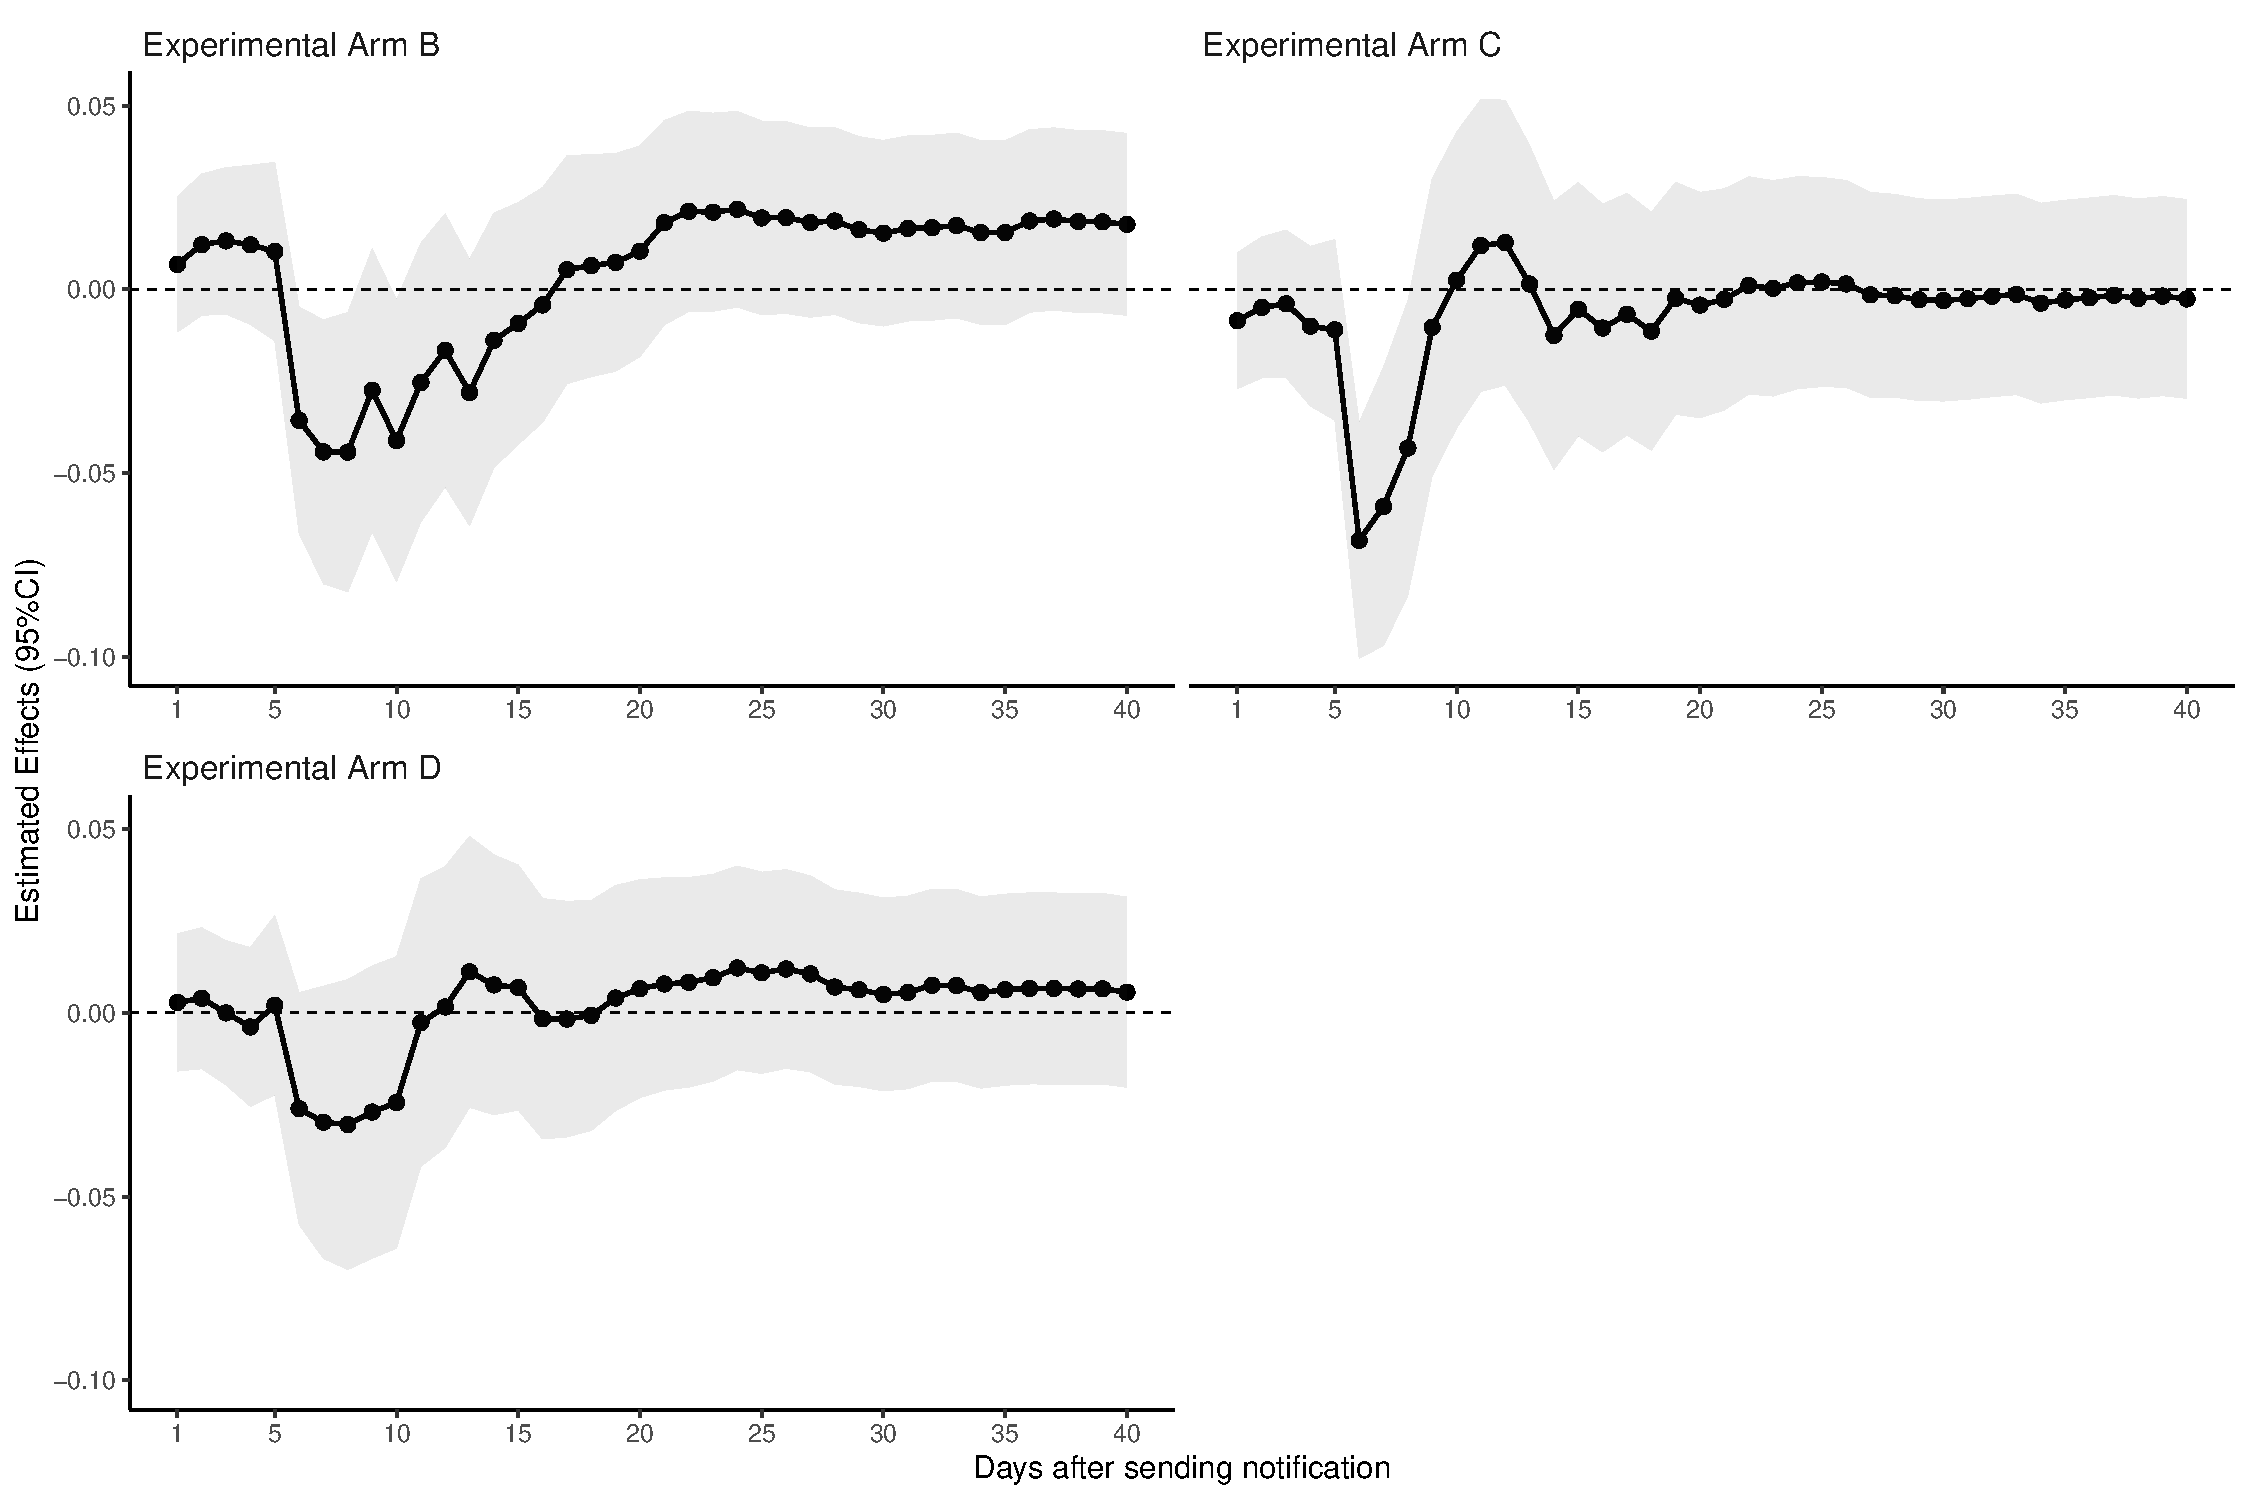
\includegraphics{JMDPRC~2/figure-latex/old-male-flow-1} \caption{Effect on Reply within Specific Days after Sending Notification among Males More than 30. Notes: These plots show the average effect (and associated 95 percent confidential interval) on cumulative responses on specific day. We use robust standard errors. We control number of past coordinations, number of hospitals per 10 square kilometers, number of hospitals with PBSC collection per 10 square kilometers, number of hospitals with BM collection per 10 square kilometers, month dummies, and week dummies.}\label{fig:old-male-flow}
\end{figure}

\begin{figure}[t]
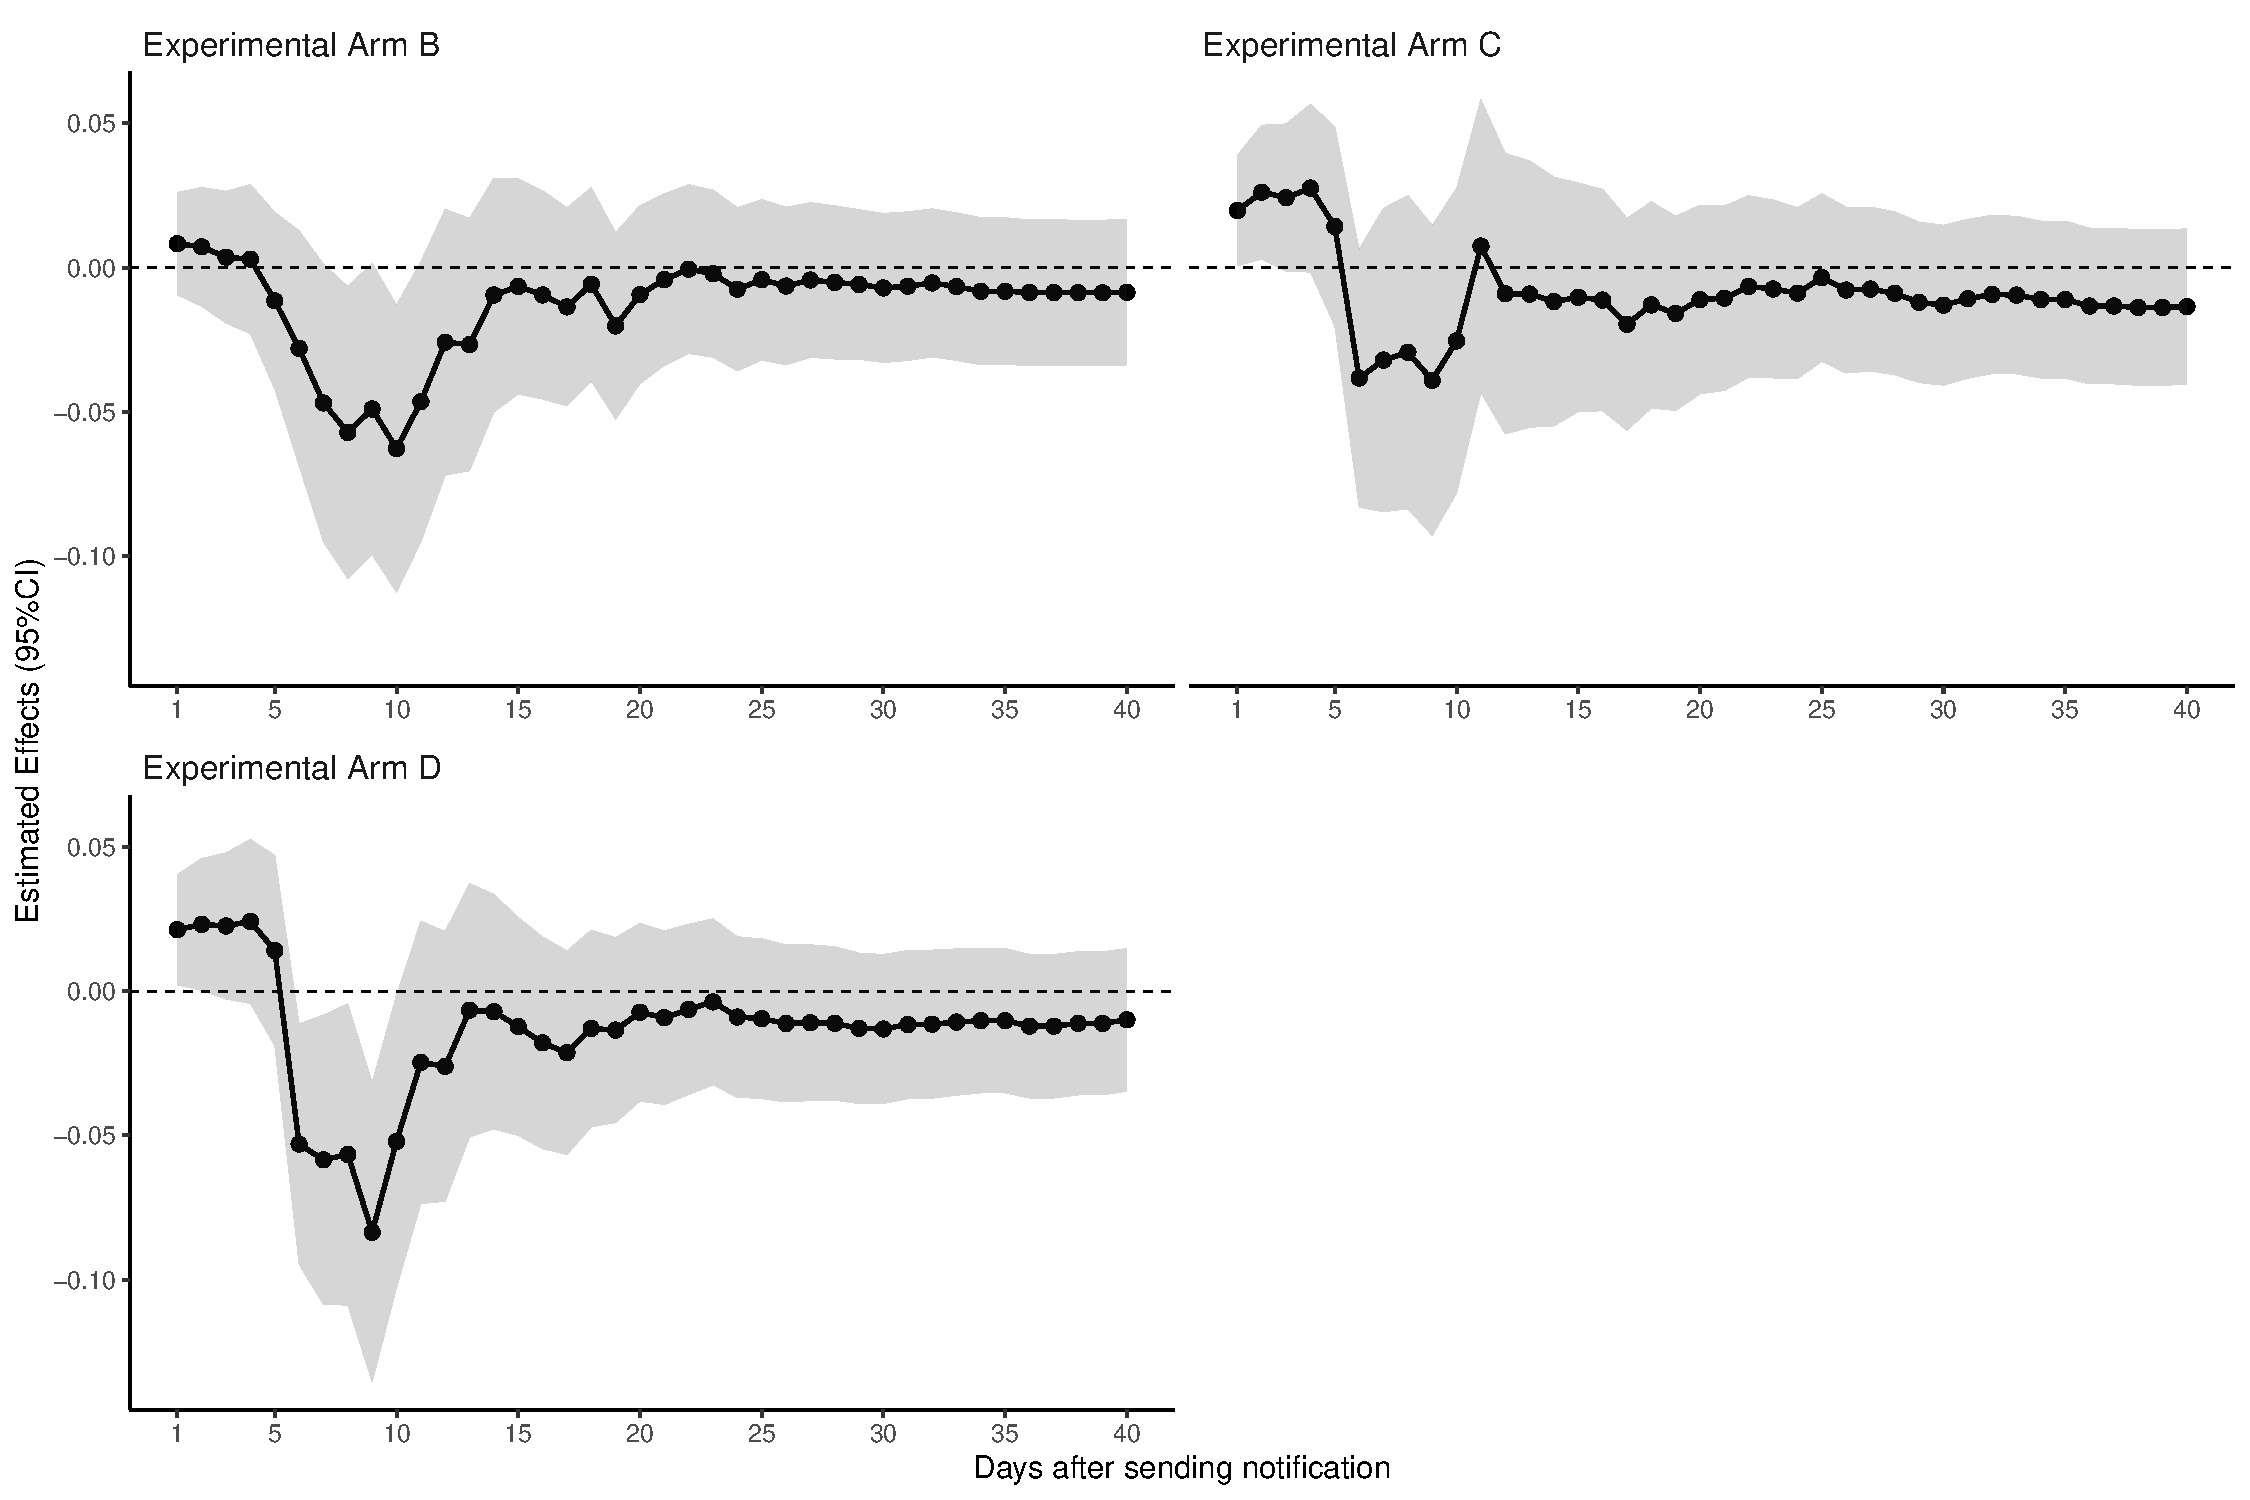
\includegraphics{JMDPRC~2/figure-latex/old-female-flow-1} \caption{Effect on Reply within Specific Days after Sending Notification among Females More than 30. Notes: These plots show the average effect (and associated 95 percent confidential interval) on cumulative responses on specific day. We use robust standard errors. We control number of past coordinations, number of hospitals per 10 square kilometers, number of hospitals with PBSC collection per 10 square kilometers, number of hospitals with BM collection per 10 square kilometers, month dummies, and week dummies.}\label{fig:old-female-flow}
\end{figure}

\begin{table}[H]

\caption{\label{tab:rcf-int-cate}Conditional Average Treatment Effect Estimated by RCF}
\centering
\fontsize{9}{11}\selectfont
\begin{threeparttable}
\begin{tabular}[t]{lcccc}
\toprule
\multicolumn{1}{c}{ } & \multicolumn{2}{c}{Female} & \multicolumn{2}{c}{Male} \\
\cmidrule(l{3pt}r{3pt}){2-3} \cmidrule(l{3pt}r{3pt}){4-5}
\multicolumn{1}{c}{ } & \multicolumn{1}{c}{Age < 30} & \multicolumn{1}{c}{30 < Age} & \multicolumn{1}{c}{Age < 30} & \multicolumn{1}{c}{30 < Age} \\
\cmidrule(l{3pt}r{3pt}){2-2} \cmidrule(l{3pt}r{3pt}){3-3} \cmidrule(l{3pt}r{3pt}){4-4} \cmidrule(l{3pt}r{3pt}){5-5}
 & (1) & (2) & (3) & (4)\\
\midrule
B & -0.0006 & -0.0090 & 0.1227*** & 0.0215\\
 & (0.0480) & (0.0286) & (0.0400) & (0.0213)\\
C & 0.0427 & -0.0148 & 0.0506 & -0.0094\\
 & (0.0481) & (0.0295) & (0.0409) & (0.0226)\\
D & -0.0548 & 0.0074 & 0.0498 & 0.0252\\
 & (0.0483) & (0.0290) & (0.0402) & (0.0220)\\
\bottomrule
\end{tabular}
\begin{tablenotes}
\item Notes: * p < 0.1, ** p < 0.05, *** p < 0.01. Standard errors are in parentheses. See Athey and Wager (2019) for estimation method of conditional average treatment effect (CATE). Since these estimates are asymptotically normal, we calculate z-score under the null hypothesis that CATE is zero, and obtain p-value. 
\end{tablenotes}
\end{threeparttable}
\end{table}

\begin{table}[H]

\caption{\label{tab:rcf-middle-male}Sample Characteristics of Predicted Treatment Effect of Arm B (Middle-aged Males)}
\centering
\fontsize{9}{11}\selectfont
\fontsize{9}{11}\selectfont
\begin{threeparttable}
\begin{tabular}[t]{lccc}
\toprule
\multicolumn{1}{c}{ } & \multicolumn{2}{c}{Predicted treatment effect} & \multicolumn{1}{c}{ } \\
\cmidrule(l{3pt}r{3pt}){2-3}
\multicolumn{1}{c}{ } & \multicolumn{1}{c}{Effect < 0.1} & \multicolumn{1}{c}{0.1 < Effect} & \multicolumn{1}{c}{P-value} \\
\cmidrule(l{3pt}r{3pt}){2-2} \cmidrule(l{3pt}r{3pt}){3-3} \cmidrule(l{3pt}r{3pt}){4-4}
 & (1) & (2) & (3)\\
\midrule
Age & 35.685 & 37.609 & < 0.001\\
Number of past coordinations & 1.664 & 2.529 & < 0.001\\
Number of listed hospitals & 0.400 & 1.441 & < 0.001\\
Number of hospitals listed with PBSC collection & 0.136 & 0.473 & < 0.001\\
Number of hospitals listed with BM collection & 0.202 & 0.848 & < 0.001\\
N & 9101 & 1948 & \\
\bottomrule
\end{tabular}
\begin{tablenotes}
\item Notes: Column (1) and (2) show average sample characteristics. Column (3) shows p-values of difference-in-means test. We use males with 30--39 age.
\end{tablenotes}
\end{threeparttable}
\end{table}

\begin{table}[H]

\caption{\label{tab:rcf-older-male}Sample Characteristics of Predicted Treatment Effect of Arm C (Older Males)}
\centering
\fontsize{9}{11}\selectfont
\fontsize{9}{11}\selectfont
\begin{threeparttable}
\begin{tabular}[t]{lccc}
\toprule
\multicolumn{1}{c}{ } & \multicolumn{2}{c}{Predicted treatment effect} & \multicolumn{1}{c}{ } \\
\cmidrule(l{3pt}r{3pt}){2-3}
\multicolumn{1}{c}{ } & \multicolumn{1}{c}{Non-positive} & \multicolumn{1}{c}{Positive} & \multicolumn{1}{c}{P-value} \\
\cmidrule(l{3pt}r{3pt}){2-2} \cmidrule(l{3pt}r{3pt}){3-3} \cmidrule(l{3pt}r{3pt}){4-4}
 & (1) & (2) & (3)\\
\midrule
Age & 48.736 & 49.868 & < 0.001\\
Number of past coordinations & 1.765 & 1.879 & 0.051\\
Number of listed hospitals & 0.557 & 0.408 & < 0.001\\
Number of hospitals listed with PBSC collection & 0.189 & 0.138 & < 0.001\\
Number of hospitals listed with BM collection & 0.311 & 0.193 & < 0.001\\
N & 9054 & 1995 & \\
\bottomrule
\end{tabular}
\begin{tablenotes}
\item Notes: Column (1) and (2) show average sample characteristics. Column (3) shows p-values of difference-in-means test. We use men over 45 years old.
\end{tablenotes}
\end{threeparttable}
\end{table}

\begin{table}[H]

\caption{\label{tab:rcf-older-female}Sample Characteristics of Predicted Treatment Effect of Arm C (Older Females)}
\centering
\fontsize{9}{11}\selectfont
\fontsize{9}{11}\selectfont
\begin{threeparttable}
\begin{tabular}[t]{lccc}
\toprule
\multicolumn{1}{c}{ } & \multicolumn{2}{c}{Predicted treatment effect} & \multicolumn{1}{c}{ } \\
\cmidrule(l{3pt}r{3pt}){2-3}
\multicolumn{1}{c}{ } & \multicolumn{1}{c}{Non-positive} & \multicolumn{1}{c}{Positive} & \multicolumn{1}{c}{P-value} \\
\cmidrule(l{3pt}r{3pt}){2-2} \cmidrule(l{3pt}r{3pt}){3-3} \cmidrule(l{3pt}r{3pt}){4-4}
 & (1) & (2) & (3)\\
\midrule
Age & 48.653 & 49.992 & < 0.001\\
Number of past coordinations & 1.667 & 1.533 & 0.039\\
Number of listed hospitals & 0.563 & 0.419 & < 0.001\\
Number of hospitals listed with PBSC collection & 0.168 & 0.157 & 0.472\\
Number of hospitals listed with BM collection & 0.302 & 0.213 & < 0.001\\
N & 9993 & 1056 & \\
\bottomrule
\end{tabular}
\begin{tablenotes}
\item Notes: Column (1) and (2) show average sample characteristics. Column (3) shows p-values of difference-in-means test. We use women over 45 years old.
\end{tablenotes}
\end{threeparttable}
\end{table}

\clearpage

\clearpage

\bibliography{biblio.bib}



\end{document}
